\documentclass[twoside]{article}
\setlength{\oddsidemargin}{0.25 in}
\setlength{\evensidemargin}{-0.25 in}
\setlength{\topmargin}{-0.6 in}
\setlength{\textwidth}{6.5 in}
\setlength{\textheight}{8.5 in}
\setlength{\headsep}{0.75 in}
\setlength{\parindent}{0 in}
\setlength{\parskip}{0.1 in}

%
% ADD PACKAGES here:
%

\usepackage{amsmath,amsfonts,amssymb,graphicx,mathtools,flexisym}
\usepackage[framemethod=TikZ]{mdframed}
\usepackage[utf8]{inputenc}
\usepackage{cancel}
\usepackage{pgfplots}
\usepackage{multicol}
\usepackage{enumitem}
\usepackage{bbm}

%
% Theorem style
%
\mdfdefinestyle{minimal}{
	topline		= false,
	rightline	= false,
	bottomline	= false,
	leftline	= false
}

\mdfdefinestyle{left}{
	topline		=false,
	rightline	=false,
	bottomline	=false
}

\mdfdefinestyle{frame}{
	topline		= true,
	rightline	= false,
	bottomline	= true,
	leftline	= false,
	shadow		= false
}

\newmdenv[style=left,frametitle=Definition]{definition}
\newmdenv[style=minimal,frametitle=Beispiel]{expl}
\newmdenv[style=frame,frametitle={\colorbox{white}{\space Korollar\space}},
    innertopmargin=0pt,
    frametitleaboveskip=-\ht\strutbox,]{cor}
\newenvironment{proof}[1][]{%
  \ifstrempty{#1}%
  {
	\mdfsetup{frametitle={\colorbox{white}{\space Beweis\space}}}
  }
  {
	\mdfsetup{frametitle={\colorbox{white}{\space Beweis #1\space}}}
  }
  \mdfsetup{style=minimal,innertopmargin=0pt,%
            linewidth=1pt,%
            frametitleaboveskip=-\ht\strutbox,}
  \begin{mdframed}[]\relax%
  }{\end{mdframed}}
  
%incomplete proof
\newenvironment{prf}[1][]{%
  \ifstrempty{#1}%
  {
	\mdfsetup{frametitle={\colorbox{white}{\space Beweis\space}}}
  }
  {
	\mdfsetup{frametitle={\colorbox{white}{\space Beweis #1\space}}}
  }
  \mdfsetup{style=minimal,innertopmargin=0pt,%
            linewidth=1pt,%
            frametitleaboveskip=-\ht\strutbox,}
  \begin{mdframed}[]\relax%
  }{\end{mdframed}}
\AtEndEnvironment{proof}{\hfill$\square$}
\newenvironment{lemma}[1][]{%
  \ifstrempty{#1}%
  {
	\mdfsetup{frametitle={\colorbox{white}{\space Lemma\space}}}
  }
  {
	\mdfsetup{frametitle={\colorbox{white}{\space #1\space}}}
  }
  \mdfsetup{style=frame,innertopmargin=0pt,%
            frametitleaboveskip=-\ht\strutbox,}
  \begin{mdframed}[]\relax%
  }{\end{mdframed}}

%
% The following commands set up the lecnum (lecture number)
% counter and make various numbering schemes work relative
% to the lecture number.
%
\newcounter{lecnum}
\renewcommand{\thepage}{\thelecnum-\arabic{page}}
\renewcommand{\thesection}{\arabic{section}}
\renewcommand{\theequation}{\thesection.\arabic{equation}}
\renewcommand{\thefigure}{\thesection.\arabic{figure}}
\renewcommand{\thetable}{\thesection.\arabic{table}}

%
% The following macro is used to generate the header.
%
\newcommand{\lecture}[4]{
   \pagestyle{myheadings}
   %\thispagestyle{plain}
   \newpage
   \setcounter{lecnum}{#1}
   \setcounter{page}{1}
   \noindent
   \begin{center}
   \framebox{
      \vbox{\vspace{2mm}
    \hbox to 6.28in { {\bf DGL IIa
    \hfill SoSe 2017} }
       \vspace{4mm}
       \hbox to 6.28in { {\Large \hfill Vorlesung #1: #2  \hfill} }
       \vspace{2mm}
       \hbox to 6.28in { {\it Dozent: #3 \hfill Mitschrift: #4} }
      \vspace{2mm}}
   }
   \end{center}
   \markboth{Vorlesung #1: #2}{Vorlesung #1: #2}

   \vspace*{4mm}
}
%
% Convention for citations is authors' initials followed by the year.
% For example, to cite a paper by Leighton and Maggs you would type
% \cite{LM89}, and to cite a paper by Strassen you would type \cite{S69}.
% (To avoid bibliography problems, for now we redefine the \cite command.)
% Also commands that create a suitable format for the reference list.
\renewcommand{\cite}[1]{[#1]}
\def\beginrefs{\begin{list}%
        {[\arabic{equation}]}{\usecounter{equation}
         \setlength{\leftmargin}{2.0truecm}\setlength{\labelsep}{0.4truecm}%
         \setlength{\labelwidth}{1.6truecm}}}
\def\endrefs{\end{list}}
\def\bibentry#1{\item[\hbox{[#1]}]}

%Use this command for a figure; it puts a figure in wherever you want it.
%usage: \fig{NUMBER}{SPACE-IN-INCHES}{CAPTION}
\newcommand{\fig}[3]{
            \vspace{#2}
            \begin{center}
            Figure \thelecnum.#1:~#3
            \end{center}
    }
% Use these for theorems, lemmas, proofs, etc.

% **** IF YOU WANT TO DEFINE ADDITIONAL MACROS FOR YOURSELF, PUT THEM HERE:

\def\R{\mathbb{R}}      	% The reals
\def\N{\mathbb{N}}
\def\C{\mathcal{C}}     	% continuous functions
\def\W{\Omega}          	% Capital omega
\def\w{\omega}          	% Lowercase omega
\def\L{\mathrm{L}}	     	% Lebesgue-integrable functions
\def\H{\mathrm{H}}
\def\esssup{\text{ess sup}} % Essential supremum
\def\iff{\Leftrightarrow}   % If and only if
\def\implies{\Rightarrow}   % Implies
\def\e{\epsilon}            % Epsilon
\def\d{\,\mathrm{d}}        % Delta
\def\cembed{\overset{\mathclap{\text{c}}}{\hookrightarrow}}
\def\dembed{\overset{\mathclap{\text{d}}}{\hookrightarrow}}

\newcommand{\overbar}[1]{\mkern 1.5mu\overline{\mkern-1.5mu#1\mkern-1.5mu}\mkern 1.5mu}
\newcommand{\einschraenkung}{\,\rule[-5pt]{0.4pt}{12pt}\,{}}

% changed commands

\renewcommand*\labelitemi{\normalfont\bfseries\textendash}
\setlist[itemize]{noitemsep, topsep=0pt}
\setlist[enumerate]{noitemsep, topsep=0pt}
\setlength{\parskip}{0pt}
\setlength{\abovedisplayskip}{0pt}
\setlength{\belowdisplayskip}{0pt}
\setlength{\abovedisplayshortskip}{0pt}
\setlength{\belowdisplayshortskip}{0pt}

\begin{document}
%\lecture{**LECTURE-NUMBER**}{**DATE**}{**LECTURER**}{**SCRIBE**}
%\footnotetext{These notes are partially based on those of Nigel Mansell.}

% **** YOUR NOTES GO HERE:
\lecture{1}{18.04.2017}{Dr. Raphael Kruse}{Frank Rehfeld}
\section{Verallgemeinerte Ableitungen im Eindimensionalen}

\textbf{Motivation}\\
$u\colon\W\to\R$ gesucht mit
\begin{align*}
	-&u^{\prime\prime}\left(x\right) = f\left(x\right) \forall x\in\Omega\\
	 &u\left(a\right) = u\left(b\right) = 0 \forall x\in\partial\Omega
\end{align*}
für ein gegebenes $f$

\textbf{Ziel}\\
Lösungsbegriff abschwächen um unstetige $f$ umzusetzen. Idee hierfür ist die Multiplikation mit Testfunktionen und anschließende partielle Integration.
\begin{equation*}
	\int_{a}^{b} u^{\prime}\left(x\right)v^{\prime}\left(x\right) + \cancel{\left[u^{\prime}\left(x\right)v\left(x\right)\right]_{a}^{b}} = \int_{a}^{b} f\left(x\right)v\left(x\right)
\end{equation*}
Somit ist nicht mehr nötig, dass $u\in\C^{2}$. Dafür zusätzliche Forderung: $u^{\prime}v^{\prime}, fv\in\L^{1}$

\lecture{2}{19.04.2017}{Dr. Raphael Kruse}{Frank Rehfeld}
\textbf{Wiederholung}\\
\begin{enumerate}
\item	
	$\begin{cases}
			u\colon\W=\left(a,b\right)\to\R\\
			\int_{\W}u^{\prime}\left(x\right)v^{\prime}\left(x\right)\,\mathrm{d}x = \int_{\W}f\left(x\right)v\left(x\right)\,\mathrm{d}x\\
			u\left(a\right)=u\left(b\right)
		\end{cases}$
\item{}
	Eigenschaften $\L^{p}$:\\
	\begin{itemize}
		\item $1\leq p <\infty \implies \L^{p}\text{ separabel}$
		\item $\L^{\infty}$ nicht separabel
		\item $1 < p <\infty, \frac{1}{p}+\frac{1}{q}=1 \implies \left(\L^{p}\right)^{\prime} \equiv \L^{q}$\\
			  $T\colon \L^{q}\to\left(\L^{p}\right)^{\prime}, \left(Tg\right)f = \int_{\W}f\left(x\right)g\left(x\right)\,\mathrm{d}x$
		\item $\left(\L^{1}\right)^{\prime}\equiv\L^{\infty}, \L^{1}\subsetneq\left(\L^{\infty}\right)^{\prime}$\\
				$\implies \L^{1}, \L^{\infty}$ sind nicht reflexiv
	\end{itemize}
\end{enumerate}

\begin{definition}
	$\L^{1}_{\text{loc}}\left(\W\right) := \left\{u\colon\W\to\R\colon u|_{K}\in\L^{1}\left(K\right)\forall K\subset\W \text{ kompakt}\right\}$\\
	Raum der lokal integrierbaren Abbildungen
\end{definition}

\begin{definition}
	$\C^{\infty}_{\text{c}}\left(\W\right) := \left\{f\colon\W\to\R\colon f\in\C^{\infty},\operatorname{supp}\left(f\right)\subset\W\text{ kompakt}\right\}$\\
	Raum der unendlich oft differenzierbaren Funktionen mit kompakten Träger\\
	$\operatorname{supp}\left(f\right):=\left\{x\in\W\colon f\left(x\right)\neq 0\right\}$\\
	\boldmath$C^{\infty}_{\text{c}}\neq \C^{\infty}_{0}$
\end{definition}

\begin{expl}
	$\W=\R^{d},d\in\mathbb{N}$\\
	Glättungskern $J\left(x\right)=\begin{cases}
		\operatorname{exp}\left(-\frac{1}{1-|x|^{2}}\right) &, |x| < 1\\
		0 &, |x| \geq 1
	\end{cases}$
\end{expl}

\begin{definition}
	$u,v\in\L^{1}_{\text{loc}}$. Es gelte
	\begin{equation*}
		\int_{\W}u\left(x\right)\phi\left(x\right)\,\mathrm{d}x = -\int_{\W}v\left(x\right)\phi^{\prime}\left(x\right)\,\mathrm{d}x \forall\phi\in\C^{\infty}_{\text{c}}
	\end{equation*}
	$u$ heißt schwache Ableitung von $v$, $v$ heißt schwach differenzierbar
\end{definition}

\textbf{??? Beispiele als Füllmaterial ???}

\textbf{Eigenschaften}:
\begin{itemize}
	\item klassisch differenzierbar $\implies$ schwach differenzierbar
	\item schwache Ableitung ist eindeutig im $\L^{1}$-Sinne
	\item übliche Eigenschaften (Linearitär,...) bleiben erhalten
\end{itemize}

\begin{lemma}
	Sei $u\in\L^{1}_{\text{loc}}$ und
	\begin{equation*}
		\int_{\W}u\left(x\right)\phi\left(x\right)\,\mathrm{d}x = 0 \forall\phi\in\C^{\infty}_{\text{c}}
	\end{equation*}
	so folgt $u=0\in\L^{1}_{\text{loc}}$.
\end{lemma}

\begin{multicols}{2}
\begin{definition}
	$J_{\e}\colon\R\to\R, J_{\e}\left(x\right)=\begin{cases}
		c_{\e}\operatorname{exp}\left(-\frac{\e^{2}}{\e^{2}-x^{2}}\right) &, x\in\left(-\e,\e\right)\\
		0 &, \text{ sonst}
	\end{cases}$\\
	$c_{\e}:=\left(\int_{\e}^{\e}\operatorname{exp}\left(-\frac{\e^{2}}{\e^{2}-x^{2}}\right)\,\mathrm{d}x\right)^{-1}$
	$J_{\e}$ ist der Standard-Glättungskern mit Träger $\left[-\e,\e\right]${}
	\begin{itemize}
		\item $J_{\e}\in\C^{\infty}_{c}\left(\W\right)$
		\item $\int_{\R}J_{\e}\left(x\right)\,\mathrm{d}x = 1$
		\item $J_{\e}\left(x\right)\geq 0 \forall x\in\R$		
	\end{itemize}
	$\implies J_{\e}$ ist Wahrscheinlichkeits-Dichte
\end{definition}
\begin{tikzpicture}
	\begin{axis}[scaled ticks=true,xmin=-1.5,xmax=1.5,ymin=0,grid=both]
		\addplot[domain=-0.99:0.99, smooth] {e^(-1/(1-x^2))/0.444};
		\addplot[domain=-0.49:0.49, style=dashed, smooth] {e^(-(1/4)/((1/4)-x^2))/0.222};
		\addplot[domain=-0.24:0.24, style=dotted, smooth] {e^(-(1/16)/((1/16)-x^2))/0.111};
	\end{axis}
\end{tikzpicture}
\end{multicols}

\lecture{3}{25.04.2017}{Dr. Raphael Kruse}{Frank Rehfeld}
\begin{definition}
	$u\colon\W=\left(a,b\right)\to\R$ außerhalb von $\W$ mit $0$ fortgesetzt\\
	$u_{\e}:=\left(J_{\e}\star u\right)\left(x\right) = \int_{\R} J_{\e}\left(x-y\right)u\left(y\right)\,\mathrm{d}y = \int_{\R}J_{\e}\left(y\right)u\left(x-y\right)\,\mathrm{d}y$\\
	heißt \underline{Glättung} oder \underline{Regularisierung}.
\end{definition}

\textbf{Eigenschaften}\\
$u\in\L^{p}\left(\W\right), \W\subset\R \text{ offenes Intervall }, p\in\left[1,\infty\right)$
\begin{enumerate}
	\item für $\e > 0$ ist $u_{\e}$ wohldefiniert
	\item $u_{\e}\in\C^{\infty}\left(\R\right)${}
	\item $\operatorname{supp}\left(u\right)\subset\W\text{ kompakt},\e\text{ klein genug}\implies u_{\e}\in\C^{\infty}_{\text{c}}$
	\item $\|u_{\e}\|_{0,p}\leq\|u\|_{0,p}$
	\item $\|u-u_{e}\|_{0,p}\to 0\text{ für }\e\to 0$
	\item $u_{e}\left(x\right)\to u\left(x\right)\text{ fast überall }$
	\item $u\in\C\left(\W\right)\implies\|u-u_{\e}\|_{\infty}\to 0$ auf jeder kompakten Teilmenge
\end{enumerate}

\begin{lemma}[Fundamentallemma der Variationsrechnung]
	Sei $u\in\L^{1}_{\text{loc}}$ und
	\begin{equation*}
		\int_{\W}u\left(x\right)\phi\left(x\right)\,\mathrm{d}x = 0 \forall\phi\in\C^{\infty}_{\text{c}}
	\end{equation*}
	so folgt $u=0\in\L^{1}_{\text{loc}}$.
\end{lemma}
\begin{proof}
	Sei $K\subset\W$ beliebig und kompakt und $w=\operatorname{sgn}\left(u\right)\mathbbm{1}_{K}$. Wäre $w\in\C^{\infty}_{\text{c}}\left(\W\right)$, dann würde gelten
	\begin{equation*}
		0 = \int_{\W}uw = \int_{\W}|u| \implies u=0\text{.}
	\end{equation*}
	Im Allgemeinen ist $w$ jedoch nicht glatt und wir müssen den Übergang zu $w_{\e}$ vollziehen. Wähle hierfür $\e_{0}<\operatorname{dist}\left(K,\partial\W\right)$. Es gilt $w_{\e}\in\C^{\infty}_{\text{c}}\forall\e\in\left(0,\e_{0}\right)$ da $\operatorname{supp}\left(w\right)$ kompakt.
	Somit gilt
	\begin{equation*}
		\int_{\W}uw_{\e} = 0\forall\e\in\left(0,\e_{0}\right)
	\end{equation*}
	und somit $\left(uw_{\e}\right)\left(x\right)\to |u\left(x\right)|$ fast überall.\\
	Weiterhin gilt $\forall x\in\W$
	\begin{align*}
		|u\left(x\right)w_{\e}\left(x\right)| &= |u\left(x\right)||\int_{\R}J_{\e}\left(x-y\right)w\left(y\right)\,\mathrm{d}y|\\
			&\leq |u\left(x\right)|\int_{\R}J_{\e}\left(x-y\right)\underbrace{|w\left(y\right)|}_{\leq 1}\,\mathrm{d}y\\
			&\leq |u\left(x\right)|
	\end{align*}
	Somit hat $|u\left(x\right)|\mathbbm{1}_{\operatorname{supp}\left(w_{\e_{0}}\right)}$ kompakten Träger und ist Majorante für $uw_{\e}$. Es folgt
	\begin{align*}
		0 &= \lim_{\e\to 0}\int_{\R}u\left(x\right)w_{\e}\left(x\right)\,\mathrm{d}x = \int_{\R}\lim_{\e\to 0}u\left(x\right)w_{\e}\left(x\right)\,\mathrm{d}x\\
			&= \int_{\W}u\left(x\right)w\left(x\right)\,\mathrm{d}x = \int_{\W}|u\left(x\right)|\,\mathrm{d}x\text{.}
	\end{align*}
	Somit folgt $u=0$ auf $K$.
\end{proof}
\begin{proof}[der Eigenschaften der Glättung]
	\begin{enumerate}
		\item Übung
		\item Übung
		\item $1=\frac{1}{p} + \frac{1}{q}, p\in\left[1,\infty\right], x\in\R$
			\begin{align*}
				|u_{\e}\left(x\right)| &\leq \int_{\R}J_{\e}\left(x-y\right)^{\frac{1}{p}+{1}{q}}|u\left(y\right)|\,\mathrm{d}y\\
					&\overset{\mathclap{\text{Hölder}}}{\leq} \hspace*{1em} \underbrace{\left(\int_{\R}J_{\e}\left(x-y\right)\,\mathrm{d}y\right)^{\frac{1}{q}}}_{=1} \left(\int_{\R}J_{\e}\left(x-y\right)|u\left(y\right)|^{p}\,\mathrm{d}y\right)^{\frac{1}{p}}\\
				\implies\|u_{\e}\|^{p}_{0,p} &= \int_{\W}|u_{\e}\left(x\right)|^{p}\,\mathrm{d}x \leq \int_{\R}|u_{\e}\left(x\right)|^{p}\,\mathrm{d}x\\
					&\leq \int_{R}\int_{\R}J_{\e}\left(x-y\right)|u\left(y\right)|^{p}\,\mathrm{d}y\,\mathrm{d}x\\
					&\overset{\mathclap{\text{Fubini}}}{=}\hspace*{1em}\int_{\R}|u\left(y\right)|^{p}\underbrace{\int_{\R}J_{\e}\left(x-y\right)\,\mathrm{d}x}_{=1}\,\mathrm{d}y\\
					&=\int_{\R}|u\left(y\right)|^{p}\,\mathrm{d}y = \int_{\W}|u\left(y\right)|^{p}\,\mathrm{d}y = \|u\|^{p}_{0,p}
			\end{align*}
		\item{}
			\begin{align*}
				|\left(u_{\e}-u\right)\left(x\right)| &= |\int_{\R}J_{\e}\left(y\right)\left(u\left(x-y\right)-u\left(x\right)\right)\,\mathrm{d}y|\\
					&\leq \text{... Hölder ...} \leq \left(\int_{\R}J_{\e}\left(y\right)|u\left(x-y\right)-u\left(x\right)|^{p}\,\mathrm{d}y\right)^{\frac{1}{p}}\\
				\implies \|u_{\e}-u\|_{0,p}^{p} &\leq \int_{\W}\int_{-\e}^{\e}J_{\e}\left(y\right)|u\left(x-y\right)-u\left(x\right)|^{p}\,\mathrm{d}y\,\mathrm{d}x\\
					&\overset{\mathclap{\text{Fubini}}}{=}\hspace*{1em} \int_{-\e}^{\e}J_{\e}\left(y\right)\int_{\W}|u\left(x-y\right)-u\left(x\right)|^{p}\,\mathrm{d}x\,\mathrm{d}y\\
					&\leq \operatorname{sup}_{y\in\left[-\e,\e\right]}\int_{\W}|u\left(x-y\right)-u\left(x\right)|^{p}\,\mathrm{d}x
			\end{align*}
			Die Behauptung folgt, da $\forall u\in\L^{p}\left(\W\right)$ gilt $\lim_{\e\to 0}\operatorname{sup}_{y\in\left[-\e,\e\right]}\int_{\W}|u\left(x-y\right)-u\left(x\right)|^{p}\,\mathrm{d}x = 0$
		\item analog
		\item $u\in\C\left(\W\right), K\subset\W$ kompakt. Wähle $\e_{0}<\operatorname{dist}\left(K,\partial\W\right)$.\\
			$K_{0} = \left[\operatorname{inf}K-\e_{0},\operatorname{sup}K+e_{0}\right]$ bleibt kompakt und somit $u$ gleichmäßig stetig auf $K_{0}$.\\
			$\implies \forall\e<\operatorname{min}\left\{\delta,\e_{0}\right\}, x\in K$ gilt
			\begin{align*}
				|u_{e}\left(x\right)-u\left(x\right)|&\leq\int_{-\e}^{\e}J_{\e}\left(y\right)\underbrace{|u\left(x-y\right)-u\left(x\right)|}_{\leq\eta}\,\mathrm{d}y\\
					&\leq \eta\int_{-\e}^{\e}J_{\e}\left(y\right)\,\mathrm{d}y = \eta
			\end{align*}
	\end{enumerate}
\end{proof}

\begin{cor}
	$u\in\L^{1}_{\text{loc}}\left(\W\right)$ schwach differenzierbar, $v,w$ schwache Ableitungen von $u$. Dann gilt
	\begin{equation*}
		v = w \text{ fast überall}
	\end{equation*}
\end{cor}
\begin{lemma}[Satz]
	$\W=\left(a,b\right),u\in\L^{1}\left(\W\right),u^{\prime}\in\L^{1}\left(\W\right)$ schwache Ableitung von $u$\\
	$\implies u$ auf $\overbar{\W}$ fast überall gleich einer absolut stetigen Funktion\\
	\begin{equation*}
		\|u\|_{\infty} \leq\frac{\operatorname{max}\left(1,b-a\right)}{b-a}\|u\|_{1,1} = \frac{\operatorname{max}\left(1,b-a\right)}{b-a}\left(\|u\|_{0,1}+\|u^{\prime}\|_{0,1}\right)
	\end{equation*}
\end{lemma}

\lecture{4}{26.04.2017}{Dr. Raphael Kruse}{Frank Rehfeld}
\begin{proof}
	\begin{equation*}
		v\left(x\right) = \int_{a}^{x}u^{\prime}\left(y\right)\,\mathrm{d}y
	\end{equation*}
	mit $u\in\L^{1}\left(\W\right)$. Somit ist $v$ absolut stetig für klassisch differenzierbare $u$ mit $u^{prime}=v^{\prime}$
	\begin{align*}
		\int_{\W}v\left(x\right)\phi\left(x\right)\,\mathrm{d}x &= -\int_{\W}v^{\prime}\left(x\right)\phi\left(x\right)\,\mathrm{d}x \\
			&= -\int_{\W}u^{\prime}\left(x\right)\phi\left(x\right)\,\mathrm{d}x = \int_{\W}u\left(x\right)\phi\left(x\right)\,\mathrm{d}x
	\end{align*}
	Mit dem vorigen Korrolar erhält man somit
	\begin{equation*}
		\exists c\in\R \colon u\left(x\right) = v\left(x\right) + c \text{ fast überall in } \W
	\end{equation*}
	Mit dem Mittelwertsatz erhält man 
	\begin{align*}
		\implies \exists x_{0}&\in\left[a,b\right] = \overbar{\W} \colon \int_{a}^{b}u\left(\xi\right)\,\mathrm{d}\xi = \left(b-a\right)u\left(x_{0}\right)\\
		\implies u\left(x\right) &= u\left(x_{0}\right) + \int_{x_{0}}^{x}u^{\prime}\left(\xi\right)\d\xi\\
			&= \frac{1}{b-a}\int_{a}^{b}u\left(\xi\right)\d\xi + \int_{x_{0}}^{x}u^{\prime}\left(\xi\right)\d\xi\\
		\implies \|u\|_{\infty} &\leq \frac{\operatorname{max}\left(1,b-a\right)}{b-a}\left(\|u\|_{0,1}+\|u^{\prime}\|_{0,1}\right)
	\end{align*}
\end{proof}

\begin{itemize}
	\item \textbf{Dieser Satz gilt nur im Eindimensionalen!}\\
	\item \textbf{Fast überall gleich einer absolut stetigen Funktion $\neq$ Fast überall absolut stetig}
\end{itemize}

\begin{definition}
	$u,v\in\L^{1}_{\text{loc}}\left(\W\right), n\in\mathbb{N}, v n$-te schwache Ableitung von $u$
	\begin{equation*}
		\int_{\W} v\left(x\right)\phi\left(x\right)\d x = \left(-1\right)^{n} \int_{\W} u\left(x\right)\phi^{\left(n\right)}\left(x\right)\d x \forall \phi\in\C^{\infty}_{\text{c}}\left(\W\right)
	\end{equation*}
	\textbf{Im höherdimensionalen ist das Fehlen von Ableitungen niedrigerer Ordnung möglich.}
\end{definition}

\begin{lemma}[Satz]
	$u\in\L^{1}\left(\W\right), n\in\mathbb{N},\W=\left(a,b\right)$\\
	$\exists n$-te schwache Ableitung $u^{\left(n\right)}\in\L^{1}\left(\W\right) \implies \exists k$-te schwache Ableitung für $k=1,\dots,n-1$ und $u^{\left(k\right)}$ ist fast überall gleich einer absolut stetigen Funktion.
\end{lemma}
\begin{proof}
	$v_{n-1}\left(x\right) = \int_{a}^{x}u^{\left(n\right)}\left(y\right)\d y$ und somit ist $v_{n-1}$ absolut stetig und damit $v_{n-1}^{\prime} = u^{\left(n\right)}$ fast überall gleich einer absolut stetigen Funktion.\\
	Rekursiv erhält man $v_{k-1}\left(x\right) = \int_{a}^{x}v_{k}\left(y\right)\d y \implies v_{k-1}$ absolut stetig und somit $v_{k-1}^{\prime} = v_{k}$ fast überall gleich einer absolut stetigen Funktion.\\
	Und somit:
	\begin{align*}
		\left(-1\right)^{n}\int_{a}^{b}u\left(x\right)\phi^{\left(n\right)}\left(x\right)\d x &= \int_{a}^{b}u^{\left(n\right)}\left(x\right)\phi\left(x\right)\d x\\
			&= \int_{a}^{b} v_{n-1}^{\prime}\left(x\right)\phi\left(x\right)\d x\\
			&= \dots = \left(-1\right)^{n}\int_{a}^{b}v_{0}\left(x\right)\phi^{\left(n\right)}\left(x\right)\d x
	\end{align*}
	Außerdem lässt sich das Korollar verallgemeinern
	\begin{equation*}
		\int_{\W}w\phi^{\left(n\right)}\d x = 0 \forall \phi\in\C_{\text{c}}^{\infty}\left(\W\right) \implies w\left(x\right) = p\left(x\right) \text{ fast überall }, p\in\mathrm{P}_{n-1}\left[x\right]
	\end{equation*}
	Und somit $u\left(x\right) = v_{0}\left(x\right) + p\left(x\right)$ ist fast überall gleich einer absolut stetigen Funktion. Da $u^{\prime}$ existiert (im klassischen Sinne falls $n\geq 2$) ist $u^{\prime}$ absolut stetig. Diese Erkenntnis kann iteriert werden.
\end{proof}

\section{Die Sobolew-Räume $\H^{1}\left(\W\right), \H^{1}_{0}\left(\W\right), \H^{-1}\left(\W\right)$}
\begin{definition}
	\begin{equation*}
		W^{k,p}\left(\W\right):=\left(u\in\L^{p}\colon\exists u^{\left(k\right)}\in\L^{p}\right)
	\end{equation*}
	ist mit
	\begin{equation*}
		\|u\|_{k,p} = \left(\sum_{j=0}^{k}\|u^{\left(j\right)}\|_{0,p}^{p}\right)^{1/p}
	\end{equation*}
	ein Banachraum, genannt Sobolewraum.
\end{definition}
\begin{definition}
	\begin{equation*}
		W^{1,2}\left(\W\right) = \H^{1}\left(\W\right)
	\end{equation*}
	ist ein Hilbertraum.
\end{definition}

\begin{lemma}[Satz]
	\begin{equation*}
		\|u\|_{1,2} = \left(u,u\right)_{1,2}^{1/2}
	\end{equation*}
	mit
	\begin{equation*}
		\left(u,v\right)_{1,2} = \left(u,v\right)_{0,2} + \left(u^{\prime},v^{\prime}\right)_{0,2} = \int uv+u^{\prime}v^{\prime}\d x
	\end{equation*}
	definiert eine Norm, bzw ein Skalarprodukt. $\left(H^{1}\left(\W\right),\|\cdot\|_{1,2},\left(\cdot,\cdot\right)_{1,2}\right)$ ist ein separabler Hilbertraum.
\end{lemma}
\begin{proof}
	\underline{Vollständigkeit}\\
	Sei $\left(u_{n}\right)_{n\in\N}$ eine Cauchy-Folge in $H^{1}$. Es gilt also:
	\begin{align*}
		u_{n}&\to u\\
		u^{\prime}_{n} &\to v
	\end{align*}
	in $\L^{2}$. Da $\W$ beschränkt ist gilt:
	\begin{equation*}
		\|u_{n}-u\|_{0,1} = \int_{\W}|u_{n}-u|\d x = \int_{W}1|u_{n}-u|\d x \overset{\mathclap{\text{C-S}}}{\leq} \int_{\W} 1\d x \|u_{n}-u\|_{0,2}
	\end{equation*}
	Mit einer Hausaufgabe folgt, dass $u$ schwach differenzierbar ist und $u^{\prime}=v$. Somit ist $u\in\H^{1}\left(\W\right)$.\\
	\underline{Separabilität}\\
	Sei $X=\L^{2}\left(\W\right)\times\L^{2}\left(\W\right), T\colon \H^{1}\left(\W\right)\to X, u\mapsto Tu=\left(u,u^{\prime}\right)$.\\
	$T$ ist wohldefiniert, linear und isometrisch. Also ist $T$ injektiv. Somit ergibt sich, dass $T\left(\H^{1}\left(\W\right)\right)\subset X$ ein Unterraum ist. Also $H^{1}\left(\W\right)\cong T\left(\H^{1}\left(\W\right)\right)$. Es folgt somit aus $\H^{1}\left(\W\right)$ vollständig, dass $T\left(\H^{1}\left(\W\right)\right)$ abgeschlossen in $X$ ist. Somit gilt:
	\begin{align*}
		\L^{2}\left(\W\right)\text{ separabel } &\implies X\text{ separabel}\\
			&\implies T\left(\H^{1}\left(\W\right)\right)\text{ separabel, da abgeschlossen}\\
			&\implies \H^{1}\left(\W\right)\text{ separabel}
	\end{align*}
\end{proof}

\lecture{5}{02.05.2017}{Dr. Raphael Kruse}{Frank Rehfeld}
\begin{definition}
	$\left(X,\|\cdot\|_{X}\right),\left(Y,\|\cdot\|_{Y}\right)$ seien Banachräume. Eine lineare, injektive Abbildung
	\begin{equation*}
		j\colon X\to Y
	\end{equation*}
	wird \textbf{Einbettung} genannt. $X$ kann also mit $j\left(X\right)$ identifiziert werden.
	\begin{itemize}
		\item Ist $j$ stetig, so sagt man, $X$ ist stetig in $Y$ eingebettet ($X\hookrightarrow Y$).
		\item Ist $j$ kompakt, so sagt man, $X$ ist kompakt in $Y$ eingebettet ($X\cembed Y$)
		\item Ist $j\left(X\right)$ dicht in $Y$ und $X\hookrightarrow Y$, so sagt man, $X$ ist dicht in $Y$ eingebettet ($X\dembed Y$)
	\end{itemize}
\end{definition}

\begin{lemma}[Satz]
	$u\in\H^{1}\left(\W\right)$ ist fast überall gleich einer absolut stetigen Funktion.\\
	$\H^{1}\left(\W\right)\cembed\C\left(\overbar{\W}\right)$
\end{lemma}
\begin{proof}
	Mithilfe der Cauchy-Schwarz-Ungleichung erhalten wir $\L^{2}\left(\W\right)\hookrightarrow\L^{1}\left(\W\right)$ und somit $\H^{1}\left(\W\right)\hookrightarrow W^{1,1}\left(\W\right)$ und somit die erste Aussage.
	
	Sei $u\in\H^{1}\left(\W\right)${}
	\begin{align*}
		\|u\|_{\infty} &\leq \frac{\operatorname{max}\left(1,b-a\right)}{b-a}\left(\int_{a}^{b}|u\left(\xi\right)|\d\xi + \int_{a}^{b}|u^{\prime}\left(\xi\right)\d\xi\right)\\
		&\overset{\mathclap{\text{CSU}}}{\leq} \hspace*{1em} \frac{\operatorname{max}\left(1,b-a\right)}{b-a}\left(\int_{a}^{b}1\d\xi\right)^{1/2}\left(\int_{a}^{b}\left(|u\left(\xi\right)|+|u^{\prime}\left(\xi\right)|\right)^{2}\d\xi\right)^{1/2}\\
		&\leq \sqrt{2}\frac{\operatorname{max}\left(1,b-a\right)}{b-a}\left(\int_{a}^{b}1\d\xi\right)^{1/2}\left(\int_{a}^{b}|u\left(\xi\right)|^{2}+|u^{\prime}\left(\xi\right)|^{2}\d\xi\right)^{1/2}\\
		&\leq \sqrt{2}\frac{\operatorname{max}\left(1,b-a\right)}{\sqrt{b-a}}\|u\|_{1,2}
	\end{align*}
	und somit haben wir $\H^{1}\left(\W\right)\hookrightarrow \C\left(\overbar{\W}\right)$.\\
	Sei $\left(u_{n}\right)\subset\H^{1}\left(\W\right)$ eine bezüglich $\|\cdot\|_{1,2}$ beschränkte Folge. Dann ist $\left(u_{n}\right)$ auch bezüglich $\|\cdot\|_{\infty}$ beschränkt. Mit
	\begin{align*}
		|u_{n}\left(x_{1}\right)-u_{n}\left(x_{2}\right)| &= \int_{\operatorname{min}}^{\operatorname{max}}u^{\prime}_{n}\left(\xi\right)\d\xi\\
			&< \sqrt{|x_{1}-x_{2}|}\underbrace{\left(\int_{\W}|u^{\prime}_{n}\left(\xi\right)|^{2}\d\xi\right)^{1/2}}_{\leq \|u\|_{1,2} \leq M}
	\end{align*}
	erhalten wir, dass $\left(u_{n}\right)$ gleichgradig stetig ist. Wir erhalten mit Arzela-Ascoli, dass $\left(u_{n}\right)$ kompakt ist und $\H^{1}\left(\W\right)\cembed\C\left(\overbar{\W}\right)$
\end{proof}

\begin{lemma}[Satz]
	$C^{\infty}\left(\W\right)$ liegt dicht in $H^{1}\left(\W\right)$.
\end{lemma}
\begin{lemma}
	$u\in\H^{1}\left(\W\right), 0<\e_{0}<\frac{b-a}{2}$.\\
	$\implies u_{\e} = J_{e}\star u\overset{\mathclap{\e\to 0}}{\rightarrow}u$ bezüglich $\|\cdot\|_{1,2}$ auf $\left(a-\e,b+\e\right)$.
\end{lemma}
\begin{proof}
	$x\in\left(a+\e_{0},b-\e_{0}\right), \e\in\left(0,\e_{0}\right)$. Es sei $\phi\colon y\mapsto J_{\e}\left(x-y\right)\in\C^{\infty}_{\text{c}}\left(\R\right)$. Dann gilt
	\begin{equation*}
		\operatorname{supp}\left(\phi\right) = \left[x-\e,x+\e\right]\subset\left(a,b\right)
	\end{equation*}
	und somit $\phi\in\C^{\infty}_{\text{c}}\left(\W\right)$. Es folgt also $\forall x\in\left(a+\e_{0},b-\e_{0}\right),\e\in\left(0,\e_{0}\right)${}
	\begin{align*}
		\left(u^{\prime}\right)_{\e}\left(x\right) &= \int_{\W}J_{\e}\left(x-y\right)u^{\prime}\left(y\right)\d y\\
			&= -\int_{\W}\frac{\partial}{\partial y}J_{\e}\left(x-y\right)u\left(y\right)\d y\\
			&\overset{\mathclap{\text{Kette}}}{=}\hspace*{1em}\left(-1\right)^{2}\int_{\W}J^{\prime}_{\e}\left(x-y\right)u\left(y\right)\d y\\
			&\overset{\mathclap{\text{Majorante}}}{=}\hspace*{1.5em}\frac{\partial}{\partial x}\int_{\W}J_{\e}\left(x-y\right)u\left(y\right)\d y = \left(u_{\e}\right)^{\prime}\left(x\right)
	\end{align*}
	Somit folgt $u_{\e}\to u$ und $\left(u^{\prime}\right)_{\e}\to u^{\prime}$ in $\L^{2}\left(a+\e_{0},b-\e_{0}\right)$.
\end{proof}
\begin{prf}[des Satzes]
	\begin{multicols}{2}
	\begin{enumerate}
		\item{}
			Seien $I_{1},I_{2},I_{3}$ offene Intervalle mit \mbox{$\bigcup_{i=1}^{3}I_{i}\supset\left[a,b\right]$}, $a\in I_{1}$,$b\in I_{3}$, $I_{2}\subset\left[a,b\right]$, $I_{1}\cap I_{3} = \emptyset$
		\item{}
			\underline{Partition der Eins}\\
			$\Psi_{i}\in\C^{\infty}_{\text{c}}\left(\R\right)$, $i=1,2,3$\\
			\mbox{$\operatorname{supp}\left(\Psi_{i}\right)\subset I_{i}$}, \mbox{$\sum_{i=1}^{3}\Psi_{i}\left(x\right)=1 \forall x\in\left[a,b\right]$}
		\item{}
			$u_{i}:=u\Psi_{i} \implies u = \sum_{i=1}^{3}u_{i}$ in $\left[a,b\right]$.\\
			Es gilt $u_{i}^{\prime} = u\Psi_{i}^{\prime}+u^{\prime}\Psi_{i}$ und somit $u^{\prime}\in\L^{2}\left(\W\right)$ und \mbox{$u_{i}\in\H^{1}\left(\W\right)$}.\\
			Wir definieren nun $v_{1}:=u_{1}\left(x+\delta\right)$ für $\delta\in\left(0,\e_{0}\right)$. Da $b\notin\operatorname{supp}\left(u_{1}\right)$ gilt
			\begin{equation*}
				v_{1}\in\H^{1}\left(a-\delta,b+\delta\right)
			\end{equation*}
			und somit 
			\begin{equation*}
				\forall\eta>0\exists\delta_{0}\leq\delta\colon\|v_{1,\e}-v_{1}\|_{1,2}<\eta\forall\e\in\left(0,\delta_{0}\right)
			\end{equation*}
		\scalebox{0.9}{\begin{tikzpicture}
			\begin{axis}[xmin=-1.5,xmax=2,ymin=0,ymax=2,grid=both,xticklabels={}]
				\addplot[domain=-1:-0.5, smooth, red] {1};
				\addplot[domain=-1.5:-1.01, smooth, red] {e^(-(1/4)/((1/4)-(x+1)^2))/0.37};
				\addplot[domain=-0.49:-0.01, smooth, red] {e^(-(1/4)/((1/4)-(x+1/2)^2))/0.37};
				\addplot[domain=0:0.5, smooth, blue] {1};
				\addplot[domain=-0.5:-0.01, smooth, blue] {e^(-(1/4)/((1/4)-(x)^2))/0.37};
				\addplot[domain=0.51:0.99, smooth, blue] {e^(-(1/4)/((1/4)-(x-1/2)^2))/0.37};
				\addplot[domain=1:1.5, smooth, green] {1};
				\addplot[domain=0.5:0.99, smooth, green] {e^(-(1/4)/((1/4)-(x-1)^2))/0.37};
				\addplot[domain=1.51:1.99, smooth, green] {e^(-(1/4)/((1/4)-(x-3/2)^2))/0.37};
			\end{axis}
		\end{tikzpicture}}
	\end{enumerate}
	\end{multicols}
\end{prf}

\lecture{6}{03.05.2017}{Dr. Raphael Kruse}{Frank Rehfeld}
\begin{proof}[Fortsetzung]
	\begin{enumerate}
		\setcounter{enumi}{3}
		\item Stetigkeit im $\L^{2}$-Mittel $\implies \forall\eta>0\exists\e_{\eta}\in\left(0,\delta\right)\colon\forall\e\in\left(0,\e_{\eta}\right)\colon\|v_{1,\e_{\eta}}-v_{1}\|_{1,2} < \eta$ in $\H^{1}\left(a,b\right)$.{}
		\item Zusammen ergibt sich für $\delta,\e$ hinreichend klein:
			\begin{equation*}
				\|v_{1,\e}-u_{1}\| \leq \|v_{1,\e}-v_{1}\|_{1,2}+\|v_{1}-u_{1}\|_{1,2}<2\eta
			\end{equation*}
		\item  $u_{3}$ wird analog approximiert, $u_{2}$ kann direkt geglättet werden
		\item $v_{\e} := \left(v_{1,\e}+v_{2,\e}+v_{3,\e}\right)\einschraenkung_{\left[a,b\right]}\in\C^{\infty}\left[a,b\right]$ mit
			\begin{equation*}
				\|v_{\e}-u\|_{1,2} \leq \sum_{i=1}^{3}\|v_{i,\e}-u_{i}\|_{1,2} < 6\eta
			\end{equation*}
	\end{enumerate}
\end{proof}

\begin{lemma}[Produktregel]
	$u\in\H^{1}\left(\W\right),\Psi\in\C^{\infty}_{\text{c}}\left(\W\right) \implies u\Psi\in\H^{1}\left(\W\right)$ und $\left(u\Psi\right)^{\prime}=u^{\prime}\Psi+u\Psi^{\prime}$
\end{lemma}
\begin{proof}
	$\Psi\in\C^{\infty}_{\text{c}}\left(\W\right)\implies u\Psi\in\L^{2}\left(\W\right)$ und $u^{\prime}\Psi+u\Psi^{\prime}\in\L^{2}\left(\W\right)$. Für $\phi\in\C^{\infty}_{\text{c}}\left(\W\right)$ gilt
	\begin{align*}
		\int_{\W}u\Psi\phi^{\prime}\d x &= \int_{\W}u\left[\left(\Psi\phi\right)^{\prime}-\Psi^{\prime}\phi\right]\d x\\
			&= -\int_{\W}u^{\prime}\left(\Psi\phi\right)\d x - \int_{\W}u\Psi^{\prime}\phi\d x\\
			&= -\int_{\W}\left(u^{\prime}\Psi-u\Psi^{\prime}\right)\phi\d x
	\end{align*}
	Zusammen folgt, dass $u\Psi\in\H^{1}\left(\W\right)$.
\end{proof}

\begin{lemma}[Satz von Rellich]
	Es gilt
	\begin{equation*}
		\H^{1}\left(\W\right)\cembed\L^{2}\left(\W\right)
	\end{equation*}
\end{lemma}
\newpage
\begin{proof}
	Es gilt $\C\left(\overbar{\W}\right)\hookrightarrow\L^{2}\left(\W\right)$, da
	\begin{align*}
		\|v\|_{0,2}^{2} &= \int_{\W}|v\left(x\right)|^{2}\d x\\
			&\leq \|v\|_{\infty}^{2}\int_{\W}1\d x\\
			&=\|v\|_{\infty}^{2}\left(b-a\right)
	\end{align*}
	Somit folgt
	\begin{equation*}
		\H^{1}\left(\W\right)\cembed\C\left(\overbar{\W}\right)\hookrightarrow\L^{2}\left(\W\right)
	\end{equation*}
\end{proof}
\begin{itemize}
	\item $\C^{k}\left(\W\right), k\geq 1$ auch dicht in $\H^{1}\left(\W\right)${}
	\item $\C^{\infty}_{\text{c}}$ \textbf{nicht} dicht in $\H^{1}\left(\W\right)$
\end{itemize}

\begin{definition}
	\begin{equation*}
		H^{1}_{0}\left(\W\right) := \overbar{\C^{\infty}_{\text{c}}\left(\W\right)}
	\end{equation*}
	wobei der Abschluss bezüglich $\|\cdot\|_{1,2}$ gebildet wird.
	
	Es gilt $\H^{1}_{0}\left(\W\right)\subsetneq\H^{1}\left(\W\right)${}
	
	Sei $\left(\phi_{n}\right)\subset\C^{\infty}_{\text{c}}\left(\W\right)$ mit $\|\phi_{n}-u\|_{1,2}\to 0$ für ein $u\in\H^{1}\left(\W\right)$. Dann hat $u$ einen absolut stetigen Repräsentanten und es gilt $\|\phi_{n}-u\|_{\infty}\to 0$ und somit $u\left(a\right)=\operatorname{lim}\phi_{n}\left(a\right)=0$ und analog $u\left(b\right)=0$.{}
\end{definition}

\begin{lemma}[Charakterisierung von $\H^{1}_{0}\left(\W\right)$]
	\begin{equation*}
		\H^{1}_{0}\left(\W\right) = \left\{u\in\H^{1}\left(\W\right)\colon u\left(a\right)=u\left(b\right)=0\right\}
	\end{equation*}
\end{lemma}

\begin{lemma}[Poincare-Friedrichs-Ungleichung]
	Sei $u\in\H^{1}_{0}\left(\W\right)$. Dann gilt $\|u\|_{0,2}\leq\frac{b-a}{\sqrt{2}}\|u^{\prime}\|_{0,2}$.
\end{lemma}
\textbf{Die Aussage gilt nicht für $H^{1}\left(\W\right)$!}
\begin{proof}
	\begin{align*}
		u\left(x\right) &= \underbrace{u\left(a\right)}_{= 0} + \int_{a}^{x}u^{\prime}\left(\xi\right)\d\xi \implies |u\left(x\right)|\leq\int_{a}^{x}|u\left(\xi\right)|\d\xi\\
		\implies \|u\|_{0,2}^{2} &\leq \int_{\W}\left(\int_{a}^{x}1|u^{\prime}\left(\xi\right)|\d\xi\right)^{2}\d x\\
			&\leq \int_{\W}\left(\int_{a}^{x}1\d\xi \int_{a}^{x}|u^{\prime}\left(\xi\right)|^{2}\d\xi\right)\d x\\
			&\leq \int_{\W}\left(x-a\right)\d x \int_{a}^{b}|u^{\prime}\left(\xi\right)|^{2}\d\xi\\
			&= \frac{1}{2}\left(b-a\right)^{2}\|u^{\prime}\|_{0,2}^{2}
	\end{align*}
\end{proof}
\begin{itemize}
	\item Die Konstante kann auf $\frac{b-a}{\pi}$ verbessert werden.
	\item $\|\cdot\|_{1,2}$ und $|\cdot|_{1,2} := \|u^{\prime}\|_{0,2}$ sind äquivalent auf $\H^{1}_{0}\left(\W\right)$.{}
	\item Auf $\H^{1}\left(\W\right)$ ist $|\cdot|_{1,2}$ nur eine Halbnorm, da sie Konstanten übersieht.
\end{itemize}

\begin{lemma}[Satz]
	$\left(\H^{1}_{0}\left(\W\right),|\cdot|_{1,2},\left[u,v\right]_{1,2}:=\int_{\W}u^{\prime}\left(\xi\right)v^{\prime}\left(\xi\right)\d\xi=\left(u^{\prime},v^{\prime}\right)_{0,2}\right)$ ist ein separabler Hilbertraum.
	
	Es gilt $\H^{1}_{0}\left(\W\right)\cembed\L^{2}\left(\W\right)$ und $\H^{1}_{0}\left(\W\right)\cembed\C\left(\overbar{\W}\right)$.
\end{lemma}

\begin{lemma}[Satz]
	$\H^{1}_{0}\left(\W\right)$ liegt dicht in $\L^{2}\left(\W\right)$. Dies folgt aus $\C^{\infty}_{\text{c}}\left(\W\right)$ dicht in $\L^{2}\left(\W\right)$.{}
	\begin{equation*}
		\C^{\infty}_{\text{c}}\left(\W\right) \subset \H^{1}_{0}\left(\W\right) \subset \L^{2}\left(\W\right){}
	\end{equation*}
\end{lemma}

\begin{definition}
	\begin{equation*}
		\H^{-1}\left(\W\right) := \left(\H^{1}_{0}\left(\W\right)\right)^{\prime}
	\end{equation*}
	\begin{itemize}
		\item $\H^{-1}\left(\W\right) \simeq \H^{1}_{0}\left(\W\right)$ mit dem Riesz'schen Darstellungssatz
		\item Gelfand-Tripel: $\H^{1}_{0}\left(\W\right)\dembed\L^{2}\left(\W\right)\simeq\left(\L^{2}\left(\W\right)\right)^{\prime}\dembed\H^{-1}\left(\W\right)$
	\end{itemize}
\end{definition}

\begin{lemma}[Satz]
	\begin{equation*}
		\|f\|_{-1,2} := \operatorname{sup}_{v\neq 0}\frac{|\left<f,v\right>|}{|v|_{1,2}}
	\end{equation*}
	definiert eine Norm auf $H^{-1}\left(\W\right)$. $\left(\H^{-1}\left(\W\right),\|\cdot\|_{-1,2}\right)$ bildet einen reflexiven Banachraum. 
	
	\begin{equation*}
		L^{2}\left(\W\right)\cembed\H^{-1}\left(\W\right){}
	\end{equation*}
	oder 
	\begin{equation*}
		\forall f\in\H^{-1}\left(\W\right)\exists u_{f}\in\L^{2}\left(\W\right)\colon\left<f,v\right>=\int_{\W}u_{f}v^{\prime}\d x \forall v\in\H^{1}_{0}\left(\W\right){}
	\end{equation*}
\end{lemma}

\lecture{7}{09.05.2017}{Dr. Raphael Kruse}{Frank Rehfeld}
\begin{proof}[der Charakterisierung von $\H^{-1}\left(\W\right)$]
	Eine Richtung wurde in der Definition schon skizziert.
	
	Sei $u\in\H^{1}\left(\W\right)$ mit $u\left(a\right)=u\left(b\right)=0$. Weiterhin sei $\delta\in\left(0,\frac{b-a}{5}\right)$.
	Wähle nun $\Psi_{\delta}\in\C^{\infty}_{\text{c}}\left(\W\right)$ so, dass
	%\begin{multicols}{2}
	\begin{enumerate}
		\item $0\leq\Psi_{\delta}\leq 1$ in $\W$
		\item $|\Psi_{\delta}^{\prime}|\leq\frac{c}{\delta}$ für $c>0$
		\item $\Psi_{\delta}\left(x\right) = \begin{cases}
			0 &, x\in\left[a,a+\delta\right]\cup\left[b-\delta,b\right]\\
			1 &, x\in\left[a+2\delta,b-2\delta\right]
		\end{cases}$
	\end{enumerate}
	%\begin{tikzpicture}
	%	\centering
	%	\begin{axis}[xmin=-2,xmax=1,ymin=0,ymax=1.5,grid=both,xticklabels={},yticklabels={}]
	%		\addplot[domain=-1:0, smooth] {1};
	%		\addplot[domain=-1.5:-1.01, smooth] {e^(-(1/4)/((1/4)-(x+1)^2))/0.37};
	%		\addplot[domain=0.01:0.5, smooth] {e^(-(1/4)/((1/4)-(x)^2))/0.37};
	%	\end{axis}
	%\end{tikzpicture}
	%\end{multicols}
	So ein $\Psi_{\delta}$ existiert, z.B. $\Psi_{\delta}\left(x\right)=\int_{a+\delta}^{x}J_{\delta/2}\left(y-\left(a+\frac{3}{2}\delta\right)\right)\d y$ auf $\left[a+\delta,a+2\delta\right]$.{}
	
	Setze nun
	\begin{align*}
		v := u\Psi_{\delta} &\implies \operatorname{supp}\left(v\right) \subset \left[a+\delta,b-\delta\right]\\
			&\implies v\in\H^{1}\left(\W\right)
	\end{align*}
	Setzt man nun $v$ außerhalb von $\W$ konstant $0$ fort, so erhält man sogar $v\in\H^{1}\left(\R\right)$.{}
	
	\textbf{TODO}
\end{proof}

\section{Variationelle Formulierung von Randwertproblemen und abstrakte Operatorgleichungen}
Gegeben ist das Randwertproblem
\begin{equation*}
	\left(P_{\text{Dir}}\right) \begin{cases}
		\text{Finde } u\in\C\left(\overbar{\W}\right)\cup\C^{2}\left(\W\right)\\
		-u^{\prime\prime}\left(x\right) + c\left(x\right)u^{\prime}\left(x\right) + d\left(x\right)u\left(x\right) = f\left(x\right) \text{ in } \W\\
		u\left(a\right)=u\left(b\right) = 0
	\end{cases}
\end{equation*}
Zur Überführung von $P_{\text{Dir}}$ in eine variationelle (schwache) Formulierung führen wir folgende Schritte durch
\begin{enumerate}
	\item Multiplikation der DGL mit hinreichend glatter Testfunktion $v$
	\item Integration des Produkts über $\W${}
	\item Term zweiter Ordnung einmal partiell integrieren
	\item Ableitungen im schwachen Sinne interpretieren
\end{enumerate}

Es ergibt sich
\begin{equation*}
	\left(V_{\text{Dir}}\right) = \begin{cases}
		\text{Finde } u\in\H^{1}_{0}\left(\W\right) \rightarrow \text{(Ansatzraum)}\\
		\int_{\W}\left(u^{\prime}v^{\prime}+cu^{\prime}v+duv\right)\d x = \int_{\W}fv\d x \forall v\in\H^{1}_{0}\left(\W\right) \rightarrow \text{(Testraum)}
	\end{cases}
\end{equation*}
Für eine sinnvolle Definition ist nötig $c,d\in\L^{\infty}\left(\W\right),f\in\H^{-1}\left(\W\right)$.{}

\begin{definition}
	Die Lösung $u\in\H^{1}_{0}\left(\W\right)$ des variationellen Problems $V_{\text{Dir}}$ wird \textbf{schwache Lösung} von $P_{\text{Dir}}$ genannt.
\end{definition}

\lecture{8}{10.05.2017}{Dr. Raphael Kruse}{Frank Rehfeld}
\underline{Randbedingungen}
\begin{enumerate}
	\item Dirichlet: $u\left(a\right)=\alpha, u\left(b\right)=\beta${}
	\item Neumann: $u^{\prime}\left(a\right)=\alpha, u^{\prime}\left(b\right)=\beta${}
	\item Robin: $c_{a}u\left(a\right) + u^{\prime}\left(a\right) = \alpha, c_{b}u\left(b\right)+u^{\prime}\left(b\right)=\beta${}
	\item periodisch: $u\left(a\right)=u\left(b\right), u^{\prime}\left(a\right)=u^{\prime}\left(b\right)$
\end{enumerate}

Inhomogene Dirichlet-Randbedingungen führen zu Problemen, da die Lösung $u\notin\H^{1}_{0}\left(\W\right)$. Es wird ein neuer Ansatzraum kreiert
\begin{align*}
	\H_{\alpha,\beta}\left(\W\right) :&= \left\{u\in\H^{1}\left(\W\right)\colon u\left(a\right)=\alpha, u\left(b\right)=\beta\right\}\\
		&= g+\H^{1}_{0}\left(\W\right), g\in\H^{1}\left(\W\right)\colon g\left(a\right)=\alpha, g\left(b\right)=\beta
\end{align*}
Es ergibt sich somit ein erstes variationelles Problem
\begin{equation*}
	\left(V_{1}\right) = \begin{cases}
		\text{Finde }u\in\H_{\alpha,\beta}\\
		a\left(u,v\right) = \left<f,v\right> \forall v\in\H^{1}_{0}\left(\W\right)
	\end{cases}
\end{equation*}
oder die alternative Form
\begin{equation*}
	\left(V_{2}\right) = \begin{cases}
		\text{Finde }u_{0}\in\H^{1}_{0}\\
		a\left(u_{0},v\right) = \left<f,v\right>-a\left(g,v\right) = \left<\tilde{f},v\right> \forall v\in\H^{1}_{0}\left(\W\right)
	\end{cases}
\end{equation*}
Die inhomogenen Dirichlet-Randbedingungen werden auch wesentliche Randbedingungen genannt, da sie die Wahl des Ansatzraums beeinflussen.

Bei Neumann-Randbedingungen ergibt sich als Ansatz- und Testraum der Raum $H^{1}\left(\W\right)$. Betrachte das Problem
\begin{equation*}
	\left(P_{\text{Neu}}\right)\begin{cases}
		\text{Finde } u\in\C^{1}\left(\overbar{\W}\right)\cap\C^{2}\left(\W\right)\\
		-u^{\prime\prime}\left(x\right) = f\left(x\right) \forall x\in\W\\
		u^{\prime}\left(a\right) = \alpha, u^{\prime}\left(b\right) = \beta
	\end{cases}
\end{equation*}
Dieses Problem ist klassisch nicht eindeutig lösbar sondern nur bis auf eine Konstante. Es ist also eine weitere Bedingung ($\int_{\W}u\d x = 0$)nötig.
Die Überführung in die variationelle Formulierung ergibt das Problem
\begin{equation*}
	\left(V_{\text{Neu}}\right) \begin{cases}
		\text{Finde } u\in\H^{1}\left(\W\right)\\
		a\left(u,v\right) = \int_{\W}u^{\prime}\left(x\right)v^{\prime}\left(x\right)\d x = \left(\alpha v\left(a\right)-\beta v\left(b\right)\right) + \left(f,v\right)_{0,2} \forall v\in\H^{1}\left(\W\right)
	\end{cases}
\end{equation*}
Die Neumann-Randbedingungen werden auch natürliche Randbedingungen genannt, da sie den größtmöglichen Ansatzraum $H^{1}\left(\W\right)$ erlauben.

Insgesamt ergibt sich das abstrakte variationelle Problem
\begin{equation*}
	\left(V\right)\begin{cases}
		\text{Finde }u\in V\\
		a\left(u,v\right) = \left<f,v\right> \forall v\in V
	\end{cases}
\end{equation*}
Hierbei ist 
\begin{itemize}
	\item $\left(V,\|\cdot\|_{V}\right)$ ein reeller Banachraum
	\item $a\colon V\times V\to\R$ linear und beschränkt im zweiten Argument ($a\left(u,\cdot\right)\in V^{\prime}$)
	\item $A\colon V \to V^{\prime}, u\mapsto a\left(u,\cdot\right)$ der zu $a$ assoziierte Operator
\end{itemize}
Es ergibt sich somit das Operator-Problem
\begin{equation*}
	\left(O\right) \begin{cases}
		\text{Finde }u\in V \text{ zu } f\in V^{\prime}\\
		A\left[u\right] = f
	\end{cases}
\end{equation*}
\begin{lemma}
	$\left(V\right)$ und $\left(O\right)$ sind äquivalent.
\end{lemma}

\lecture{9}{16.05.2017}{Dr. Raphael Kruse}{Frank Rehfeld}
\section{Lineare Variationsprobleme mit stark positiver Bilinearform}
\begin{definition}
	Sei $\left(V,\|\cdot\|_{V}\right)$ ein reeller Banachraum, $a\colon V\times V\to\R, A\colon V\to V^{\prime}$ der assoziierte Operator.
	\begin{itemize}
		\item $a$ ist \textbf{bilinear}, wenn es linear in beiden Eingängen ist.
		\item $a$ bzw $A$ ist \textbf{symmetrisch}, wenn gilt $a\left(v,u\right) = a\left(u,v\right)$ bzw $\left<Av,u\right>=\left<Au,v\right>$.{}
		\item $a$ bzw $A$ ist \textbf{positiv}, wenn gilt $a\left(u,u\right)\geq 0$ bzw $\left<Au,u\right>\geq 0$
		\item $a$ bzw $A$ ist \textbf{stark positiv}, wenn gilt $a\left(u,u\right) > 0$ bzw $\left<Au,u\right> > 0$
		\item $a$ ist \textbf{beschränkt}, wenn gilt: $\exists\beta >0\colon |a\left(u,v\right)|\leq\beta\|u\|_{V}\|v\|_{V}$
		\item $A$ ist \textbf{beschränkt}, wenn es beschränkte Mengen auf beschränkte Mengen abbildet.
	\end{itemize}
\end{definition}

\begin{lemma}
	Sei $\left(V,\|\cdot\|_{V}\right)$ ein reeller Banachraum, $a\colon V\times V\to\R$ und $A\colon V\to V^{\prime}$ der assoziierte Operator.
	Es gilt
	\begin{itemize}
		\item $A$ linear $\Leftrightarrow a$ bilinear
		\item $A$ symmetrisch $\Leftrightarrow a$ symmetrisch
		\item Sei $a$ bilinear. $A$ beschränkt $\Leftrightarrow a$ beschränkt
		\item $A$ stark positiv $\Leftrightarrow a$ stark positiv
	\end{itemize}
\end{lemma}

\begin{definition}
	Sei $a\colon V\times V\to\R$ eine symmetrische, stark positive Bilinearform, $V$ Hilbertraum, $f\in V^{\prime}$. 
	\begin{align*}
		J\colon V &\to\R \\
			v &\mapsto J\left[v\right] := \frac{1}{2}a\left(v,v\right) - \left<f,v\right>
	\end{align*}
	heißt \textbf{Energiefunktional}.
\end{definition}

\begin{lemma}[Satz von Lax-Milgram]
	Sei $\left(V,\left(\cdot,\cdot\right),\|\cdot\|_{V}\right)$ ein reeller Hilbertraum, $a\colon V\times V\to\R$ eine beschränkte, stark positive Bilinearform.
	Dann besitzt das Variationsproblem $\left(V\right)$ für alle $f\in V^{\prime}$ eine eindeutige Lösung.
	
	\textbf{Es wird keine Symmetrie von $a$ gefordert.}
\end{lemma}
\begin{proof}
	\begin{enumerate}
		\item Da $a$ beschränkt ist, ist $A\colon V\to V^{\prime}$ ein lineares, stark positives Funktional.
		\item Mit dem Rieszschen Darstellungssatz gilt $V\simeq V^{\prime}$ mit $I\colon V^{\prime}\to V$.
		\item Sei $u_{0}\in V, \tau\in\left(0,\infty\right)$ beliebig. Wir definieren die Folge
			\begin{equation*}
				u^{\left(n+1\right)} = u^{\left(n\right)} + \tau I\left(f-Au^{\left(n\right)}\right) = \Phi\left(u^{\left(n\right)}\right)
			\end{equation*}
		\item $\Phi\left(u\right) = u \Leftrightarrow u = u + \tau I\left(f-Au\right)${}
		\item Seien $v,w\in V$ beliebig. Dann gilt
			\begin{align*}
				\|\Phi\left(u\right)-\Phi\left(v\right)\|_{V}^{2} &= \|v-w-\tau IA\left(v-w\right)\|_{V}^{2}\\
					&= \|v-w\|_{V}^{2} - 2\tau\left(v-w,IA\left(v-w\right)\right)_{V} + \tau^{2}\|IA\left(v-w\right)\|_{V}^{2}\\
					&= \|v-w\|_{V}^{2} - 2\tau\left<A\left(v-w\right),v-w\right> + \tau^{2}\|A\left(v-w\right)\|_{V}^{2}\\
					&\leq \|v-w\|_{V}^{2} - 2\tau \underbrace{a\left(v-w,v-w\right)}_{\geq \mu\|v-w\|_{V}^{2}} + \tau^{2}\beta^{2}\|v-w\|_{V}^{2}\\
					&\leq \left(1-2\tau\mu + \tau^{2}\beta^{2}\right)\|v-w\|_{V}^{2}
			\end{align*}
			Für $\tau\in\left(0,\frac{2\mu}{\beta^{2}}\right)$ gilt $\Phi$ ist eine Kontraktion und besitzt somit mit dem Banachschen Fixpunktsatz einen Fixpunkt.
	\end{enumerate}
\end{proof}

\begin{lemma}[Korollar]
	Unter den Voraussetzungen von Lax-Milgram gilt:
	\begin{equation*}
		A\text{ bijektiv}\Leftrightarrow A^{-1}\colon V^{\prime}\to V\text{ linear, beschränkt und stark positiv}
	\end{equation*}
\end{lemma}

\lecture{10}{17.05.2017}{Dr. Raphael Kruse}{Frank Rehfeld}
\begin{expl}
	Das klassische Problem
	\begin{equation*}
		\left(P_{2}\right)\begin{cases}
			-u^{\prime\prime}\left(x\right) = \delta_{0}\left(x\right)\text{ in }\W=\left(-1,1\right)\\
			u\left(-1\right) = u\left(1\right) = 0
		\end{cases}
	\end{equation*}
	ergibt das variationelle Problem
	\begin{equation*}
		\left(V_{2}\right)\begin{cases}
			\text{Finde } u\in\H^{1}_{0}\left(\W\right)\\
			\int_{-1}^{1} u^{\prime}\left(x\right)v^{\prime}\left(x\right)\d x = v\left(0\right) \forall v\in\H^{1}_{0}
		\end{cases}
	\end{equation*}
	Hierbei ist $a\left(u,v\right)=\int_{-1}^{1}u^{\prime}\left(x\right)v^{\prime}\left(x\right)\d x$ ein inneres Produkt und erfüllt somit die Voraussetzungen von Lax-Milgram an $a$. Außerdem gilt $|v\left(0\right)|\leq\|v\|_{\infty}\leq c\|v\|_{1,2}$ und somit ist die rechte Seite stetig. Somit sind alle Voraussetzungen von Lax-Milgram erfüllt und es existiert eine eindeutige Lösung von $\left(V_{2}\right)$.
\end{expl}
\begin{expl}
	\begin{equation*}
		\left(P_{3}\right)\begin{cases}
			-u^{\prime\prime}\left(x\right)-u\left(x\right) = f\left(x\right)\text{ in }\W=\left(0,\pi\right)\\
			u\left(-1\right) = u\left(\pi\right) = 0
		\end{cases}
	\end{equation*}
	mit $f\in\H^{-1}$ beliebig.
	\begin{equation*}
		\left(V_{3}\right)\begin{cases}
			\text{Finde } u\in\H^{1}_{0}\left(\W\right)\\
			\int_{0}^{\pi} u^{\prime}\left(x\right)v^{\prime}\left(x\right)-u\left(x\right)v\left(x\right)\d x = \left<f,v\right> \forall v\in\H^{1}_{0}
		\end{cases}
	\end{equation*}
	Hierbei ist $a$ bilinear und beschränkt. Es gilt jedoch für $v\left(x\right)=\operatorname{sin}\left(x\right)${}
	\begin{equation*}
		a\left(v,v\right) = \int_{0}^{\pi} \operatorname{cos}^{2}\left(x\right)-\operatorname{sin}^{2}\left(x\right)\d x = 0
	\end{equation*}
	Somit ist $a$ nicht stark positiv und der Satz von Lax-Milgram nicht anwendbar.
	
	In der Tat gibt es für $f\equiv 1$ keine schwache Lösung und für $f\equiv 0$ existieren unendlich viele Lösungen.
\end{expl}
\begin{lemma}[Korollar]
	Sei $V=\H^{1}_{0}\left(\W\right), f\in\H^{-1}\left(\W\right), c,c^{\prime},d\in\L^{\infty}\left(\W\right)$ und $\underline{d}\colon d\left(x\right)-\frac{1}{2}c^{\prime}\left(x\right) \geq \underline{d} > -\frac{\pi^{2}}{\left(b-a\right)^{2}}$ fast überall. Dann besitzt $\left(P_{\text{Dir}}\right)$ genau eine schwache Lösung $u\in\H^{1}_{0}\left(\W\right)$.
\end{lemma}

\begin{lemma}[Regularitätsfrage für Randwertprobleme]
	Unter Voraussetzungen des obigen Korollars und der zusätzlichen Annahme $c,d\in\C^{k-1}\left(\W\right)$ für ein $k\in\N$, $f,f^{\prime},\dots,f^{\left(k-1\right)}\in\L^{2}\left(\W\right)$ ergibt sich, für die schwache Lösung $u\in\H^{1}_{0}\left(\W\right)\cap\H^{k+1}\left(\W\right)$ und
	\begin{equation*}
		\exists C\in\left(0,\infty\right)\colon\|u\|_{\H^{k+1}\left(\W\right)}\leq C\|f\|_{\H^{k-1}\left(\W\right)}
	\end{equation*}
\end{lemma}
\begin{proof}
	\underline{Beweis für den Fall $k=1$}
	Definiere
	\begin{equation*}
		w:= -\left(f-cu^{\prime}-du\right)\in\L^{2}\left(\W\right)
	\end{equation*}
	Weiterhin sei $\psi\in\C^{\infty}_{\text{c}}\left(\W\right)\subset\H^{1}_{0}\left(\W\right)$ beliebig. Es gilt
	\begin{align*}
		a\left(u,\phi\right) &= \int_{\W}\left(u^{\prime}\phi^{\prime}+cu^{\prime}\phi + du\phi\right)\d x = \int_{\W}f\phi\d x\\
		\Leftrightarrow \int_{\W}u^{\prime}\phi^{\prime}\d x &= -\int_{\W}-\left(f\phi-cu^{\prime}\phi-du\phi\right)\d x\\
			&= -\int_{\W}-\underbrace{\left(f-cu^{\prime}-du\right)}_{=w}\phi\d x
	\end{align*}
	und somit $u\in\H^{2}\cap\H^{1}_{0}\left(\W\right)$.{}
	
	Weiterhin
	\begin{align*}
		\int_{\W}|u^{\prime\prime}|^{2}\d x &= \int_{\W}|w|^{2}\d x \\
			&\leq C\left(\|f\|_{0,2}^{2}+\|c\|_{\infty}^{2}|u|_{1,2}^{2}+\|d\|_{\infty}^{2}\|u\|_{0,2}^{2}\right)\\
			&\leq C\left(\|f\|_{0,2}^{2} + \left(\|c\|_{\infty}^{2}+\|d\|_{\infty}^{2}\frac{\left(b-a\right)^{2}}{\pi^{2}}\right)|u|_{1,2}^{2}\right)
	\end{align*}
	und mit $u=A^{-1}f$ und $\|A^{-1}\|_{L\left(\H^{-1},\H^{1}_{0}\right)} <\infty$ ergibt sich
	\begin{equation*}
		|u|_{1,2} \leq |A^{-1}f| \leq \|A^{-1}\|\|f\|_{0,2}
	\end{equation*}
\end{proof}

\begin{lemma}[Korollar]
	Unter den Voraussetzungen des Regularitätssatzes und der zusätzlichen Annahme $f\in\C\left(\overbar{\W}\right)$ mit $k=1$ gilt, dass $u$ eine Lösung im klassischen Sinne ist.
\end{lemma}
\begin{proof}
	Sei $u\in\H^{2}\left(\W\right)$. Dann besitzt $u^{\prime}\in\H^{1}\left(\W\right)$ einen stetigen Repräsentanten.
	
	Setze $w = -\left(f-cu^{\prime}-du\right)\in\C\left(\overbar{\W}\right)$. Betrachten wir nun das Problem
	\begin{equation*}
		\begin{cases}
			-\tilde{u}^{\prime\prime} = w\\
			\tilde{u}\left(a\right) = \tilde{u}\left(b\right)=0
		\end{cases}
	\end{equation*}
	Es gilt $\tilde{u} = u$ fast überall.
\end{proof}

\lecture{11}{23.05.2017}{Dr. Raphael Kruse}{Frank Rehfeld}
Es stellt sich die Frage, ob der Satz von Lax-Milgram auch auf Banachräume anwendbar ist. Hierbei unterscheiden wir 2 Fälle.
\begin{enumerate}
	\item $a$ ist symmetrisch. \\
	Dann ist $a$ ein Skalarprodukt. Nun führen wir über das Skalarprodukt eine Norm ein und erhalten, dass diese äquivalent zur Energienorm ist. Betrachte nun den Raum $\left(V,\|\cdot\|_{a},a\left(\cdot,\cdot\right)\right)$. Dieser ist ein Hilbertraum und wir können Lax-Milgram anwenden.
	\item $a$ allgemein.\\
	Hierbei betrachten wir den symmetrischen Anteil $\tilde{a}\left(u,v\right) = \frac{1}{2}\left(a\left(u,v\right)+a\left(v,u\right)\right)$. Dann ist $\tilde{a}$ symmetrisch, bilinear, beschränkt und stark positiv. Somit ist $\tilde{a}$ ein Skalarprodukt und wir können wie im obigen Fall weiter machen.
\end{enumerate}
Somit kann nicht auf jeden Banachraum der Satz von Lax-Milgram angewendet werden. Zusätzliche Anforderungen an $a$ geben die benötigte Struktur.

\section{Nicht-lineare Variationsprobleme mit stark monotonen Operatoren}
Betrachte das Problem
\begin{equation*}
	\left(P_{\text{Mon}}\right)\begin{cases}
		-\left(\Psi\left(|u^{\prime}\left(x\right)|\right)u^{\prime}\left(x\right)\right)^{\prime} + c\left(x\right)u^{\prime}\left(x\right) + d\left(x\right)u\left(x\right) = f\left(x\right) \text{ für } x\in\W=\left(a,b\right)\\
		u\left(a\right)=u\left(b\right) = 0
	\end{cases}
\end{equation*}
mit $-\left(\Psi\left(|u^{\prime}\left(x\right)|\right)u^{\prime}\left(x\right)\right)^{\prime}$ nicht-linear (genauer: quasi-linear). An $\Psi\colon\left[0,\infty\right)\to\R$ stetig haben wir folgende Anforderungen
\begin{enumerate}
	\item $|\Psi\left(t\right)|\leq M \forall t\geq 0$
	\item $|\Psi\left(t\right)t-\Psi\left(s\right)s|\leq M|t-s| \forall t,s\in\left[0,\infty\right)${}
	\item $\Psi\left(t\right)t-\Psi\left(s\right)s\geq m\left(t-s\right) \text{ für } t\geq s\geq 0$\\
			$\implies \Psi\left(t\right) \geq m \forall t\in\left[0,\infty\right)$
\end{enumerate}
Diese Modelle werden beispielsweise in der nichtlinearen Elastizitätstheorie angewandt.

\begin{definition}
	Sei $\left(V,\|\cdot\|_{V}\right)$ ein reeller Banachraum und $A\colon V\to V^{\prime}$ \textbf{Lipschitz-stetig}, dh
	\begin{equation*}
		\|A\left[u\right]-A\left[v\right]\|_{V^{\prime}}\leq\beta\|u-v\|_{V}\text{ für ein }\beta\in\left(0,\infty\right)
	\end{equation*}
	\begin{itemize}
		\item $A$ heißt \textbf{monoton} $\Leftrightarrow \left<A\left[u\right]-A\left[v\right],u-v\right> \geq 0$
		\item $A$ heißt \textbf{stark monoton} $\Leftrightarrow \exists\mu\in\left(0,\infty\right)\colon\left< A\left[u\right]-A\left[v\right],u-v\right> \geq \mu\|u-v\|_{V}^{2}$
	\end{itemize}
\end{definition}

\begin{lemma}[Satz von Zarantonello]
	Sei $\left(V,\|\cdot\|_{V},\left(\cdot,\cdot\right)_{V}\right)$ ein reeller Hilbertraum, $A\colon V\to V^{\prime}$ Lipschitz-stetig und stark monoton.
	Dann hat für jedes $f\in V^{\prime}$ das Problem $A\left[u\right] = f$ eine eindeutige Lösung.
\end{lemma}
\begin{proof}
	Der Beweis folgt in den Schritten 1. bis 4. analog dem Beweis von Lax-Milgram.
	\begin{enumerate}
		\setcounter{enumi}{4}
		\item \begin{align*}
			\|\Psi\left(v\right)-\Psi\left(w\right)\|_{V}^{2} &= \|v-w\|_{V}^{2}-2\tau\left(I\left(A\left[v\right]-A\left[w\right]\right),v-w\right) + \tau^{2}\|I\left(A\left[v\right]-A\left[w\right]\right)\|_{V}^{2}\\
			&= \|v-w\|_{V}^{2} - 2\tau\left<A\left[v\right]-A\left[w\right],v-w\right> + \tau^{2}\|A\left[v\right]-A\left[w\right]\|_{V^{\prime}}^{2}\\
			&\overset{\mathclap{\text{Monoton}}}{\leq}\left(1-2\tau\mu+\tau^{2}\beta^{2}\right)\|v-w\|_{V}^{2}
			\end{align*}
	\end{enumerate}
\end{proof}
Hiermit ist auch gezeigt, dass $A^{-1}\colon V^{\prime}\to V$ existiert. Weiterhin kann gezeigt werden, dass $A^{-1}$ Lipschitz-stetig und stark monoton ist.

\begin{lemma}[Korollar]
	Sei $V=\H^{1}_{0}\left(\W\right)$, $f\in V^{\prime}, c,c^{\prime},d\in\L^{\infty}\left(\W\right)$ und für ein $\underline{d}\in\R$ gilt
	\begin{equation*}
		d\left(x\right)-\frac{1}{2}c^{\prime}\left(x\right)\geq\underline{d}\geq -\frac{m\pi^{2}}{\left(b-a\right)^{2}} \text{ fast überall in } \W
	\end{equation*}
	Dann besitzt das Problem $A[u]=f$ genau eine Lösung, wenn $\Psi$ die Eigenschaften vom Anfang der Vorlesung erfüllt.
\end{lemma}
\begin{prf}
	Wir zeigen, dass unter den Voraussetzungen $A$ stark monoton und Lipschitz-stetig ist.
	
	Seien $c\equiv d\equiv 0$. Ansonsten folge dem linearen Fall.
	
	\underline{Lipschitz-Stetigkeit}
	
	Seien $u,v,w\in V$.
	\begin{align*}
		|\left<A\left[u\right]-A\left[v\right],w\right>| &= |a\left(u,w\right)-a\left(v,w\right)|\\
			&= |\int_{\W}\left(\Psi\left(|u^{\prime}|\right)u-\Psi\left(|v^{\prime}|\right)v\right)w\d x|\\
			&\overset{\mathclap{\text{CSU}}}{\leq}\hspace*{0.5em}\left(\int_{\W}|\Psi\left(|u^{\prime}|\right)u^{\prime}-\Psi\left(|v^{\prime}|\right)v^{\prime}|^{2}\d x\right)^{1/2} + |w|_{1,2}
	\end{align*}
	Aus Voraussetzung 2. vom Anfang der Vorlesung folgt $\forall x\in\W\colon u^{\prime}\left(x\right)v^{\prime}\left(x\right)\geq 0$
	\begin{equation*}
		|\Psi\left(|u^{\prime}\left(x\right)|\right)u^{\prime}\left(x\right)-\Psi\left(|v^{\prime}\left(x\right)|\right)v^{\prime}\left(x\right)|\leq M|u^{\prime}\left(x\right)-v^{\prime}\left(x\right)|
	\end{equation*}
	und $\forall x\in\W\colon u^{\prime}\left(x\right)\geq 0, v^{\prime}\left(x\right)<0$ folgt
	\begin{align*}
		|\Psi\left(|u^{\prime}\left(x\right)|\right)u^{\prime}\left(x\right)-\Psi\left(|v^{\prime}\left(x\right)|\right)v^{\prime}\left(x\right)| &\leq |\Psi\left(|u^{\prime}\left(x\right)|\right)u^{\prime}\left(x\right)| + |\Psi\left(|v^{\prime}\left(x\right)|\right)v^{\prime}\left(x\right)|\\
		&\leq \underbrace{\Psi\left(|u^{\prime}\left(x\right)|\right)}_{\leq M}u^{\prime}\left(x\right) + \underbrace{\Psi\left(|v^{\prime}\left(x\right)|\right)}_{\leq M}|v^{\prime}\left(x\right)|\\
		&\leq M\left(u^{\prime}\left(x\right)-|v^{\prime}\left(x\right)|\right) \leq M\left(u^{\prime}\left(x\right)-v^{\prime}\left(x\right)\right) = M|u^{\prime}\left(x\right)-v^{\prime}\left(x\right)|
	\end{align*}
	Der Fall $u^{\prime}\left(x\right)< 0, v^{\prime}\left(x\right)\geq 0$ folgt analog.
\end{prf}

\lecture{12}{24.05.2017}{Dr. Raphael Kruse}{Frank Rehfeld}
\begin{proof}[Fortsetzung]
	\underline{starke Monotonie}
	
	Betrachte
	\begin{equation*}
		\left<A\left[u\right]-A\left[v\right],u-v\right> = \int_{\W}\left(\Psi\left(|u^{\prime}|\right)u^{\prime}-\Psi\left(|v^{\prime}|\right)v^{\prime}\right)\left(u^{\prime}-v^{\prime}\right)\d x
	\end{equation*}
	Wir unterscheiden die Fälle
	\begin{enumerate}
		\item $x\in\W\colon u^{\prime}\left(x\right)\geq v^{\prime}\left(x\right)\geq 0$: Mit Eigenschaft 3. folgt
		\begin{equation*}
			\left(\Psi\left(|u^{\prime}\left(x\right)|\right)u^{\prime}\left(x\right) - \Psi\left(|v^{\prime}\left(x\right)|\right)v^{\prime}\left(x\right)\right)\left(u^{\prime}\left(x\right)-v^{\prime}\left(x\right)\right) \geq m\left(u^{\prime}\left(x\right)-v^{\prime}\left(x\right)\right)^{2}
		\end{equation*}
		\item $x\in\W\colon v^{\prime}\left(x\right)\geq u^{\prime}\left(x\right)\geq 0$ folgt analog mit vertauschten Rollen
		\item $x\in\W\colon v^{\prime}\left(x\right)\leq u^{\prime}\left(x\right)\leq 0$ und $x\in\W\colon u^{\prime}\left(x\right)\leq v^{\prime}\left(x\right)\leq 0$ folgen analog
		\item $x\in\W\colon v^{\prime}\left(x\right)\leq 0 \leq u^{\prime}\left(x\right)${}
		\begin{align*}
			&\left(\Psi\left(|u^{\prime}\left(x\right)|\right)u^{\prime}\left(x\right)-\Psi\left(|v^{\prime}\left(x\right)|\right)v^{\prime}\left(x\right)\right)\left(u^{\prime}\left(x\right)-v^{\prime}\left(x\right)\right)\\ 
			= &\underbrace{\Psi\left(-u^{\prime}\left(x\right)\right)}_{\geq m}\underbrace{u^{\prime}\left(x\right)}{\leq 0}\underbrace{\left(u^{\prime}\left(x\right)-v\left(x\right)\right)}_{\leq 0} - \underbrace{\Psi\left(-v^{\prime}\left(x\right)\right)}_{\geq m}\underbrace{v^{\prime}\left(x\right)}{\geq 0}\underbrace{\left(u^{\prime}\left(x\right)-v\left(x\right)\right)}_{\geq 0} \\
			\geq &m\left(u^{\prime}\left(x\right)-v^{\prime}\left(x\right)\right)^{2}
		\end{align*}
		\item $x\in\W\colon u^{\prime}\left(x\right)\leq 0 \leq v^{\prime}\left(x\right)$ analog zu 4.
	\end{enumerate}
	Somit ist $\Psi$ stark monoton.
\end{proof}

\textbf{Für nichtlineare Probleme ist kein allgemein gültiger Regularitätssatz bekannt.}

\begin{lemma}[Eindeutigkeit]
	$A\colon V\to V^{\prime}$ stark monoton $\implies A$ injektiv.
\end{lemma}
\begin{proof}
	Seien $v_{1},v_{2}\in V\colon A\left[v_{1}\right] = A\left[v_{2}\right]$. Dann gilt
	\begin{equation*}
		0 = \left<A\left[v_{1}\right]-A\left[v_{2}\right],v_{1}-v_{2}\right> \geq \mu\|v_{1}-v_{2}\|^{2}
	\end{equation*}
	Somit folgt $v_{1}=v_{2}$.
\end{proof}

\section{Galerkin-Verfahren und FEM}
\begin{definition}
	Sei $\left(V,\|\cdot\|_{V}\right)$ ein reeller Banachraum und $\left(V_{m}\right)_{m\in\N}$ eine Folge von endlichdimensionalen Teilräumen. $\left(V_{m}\right)$ heißt \textbf{Galerkin-Schema}, falls $\lim_{m\to\infty} \operatorname{d}\left(v,V_{m}\right) = 0 \forall v\in V$. Diese Eigenschaft wird \textbf{limitierte Vollständigkeit} genannt.
\end{definition}

\begin{definition}
	Sei $\left(\phi_{j}\right)_{j\in I}\subset V$, $I\subset \N$ mit
	\begin{itemize}
		\item je endlich viele Elemente von $\left(\phi_{j}\right)$ sind linear unabhängig
		\item $V_{m} := \operatorname{span}\left\{\phi_{1},\dots,\phi_{m}\right\}, m\in I$, ist ein Galerkin-Schema
	\end{itemize}
	Dann wird $\left(\phi_{j}\right)$ \textbf{Galerkin-Basis} von $V$ genannt.
\end{definition}

\begin{lemma}
	Sei $V$ ein reeller, separabler Banachraum. Dann besitzt $V$ eine Galerkin-Basis.
\end{lemma}
\begin{proof}
	\begin{enumerate}
		\item $\operatorname{dim} V<\infty$: Dann ist jede Basis von $V$ eine Galerkin-Basis.
		\item $\operatorname{dim} V=\infty$: Da $V$ separabel ist existiert eine dichte Teilmenge $\left(\psi_{j}\right)_{j\in\N}$.\\
			Setze nun
			\begin{align*}
				\phi_{1} :&= \psi_{1} & V_{1} &= \operatorname{span}\left\{\phi_{1}\right\}\\
				\phi_{m} :&= \psi_{j\left(m\right)} & j\left(m\right) &= \operatorname{min}\left\{j\in\N\colon \psi_{j}\notin V_{m-1}\right\}
			\end{align*}
			und es folgt
			\begin{equation*}
				\left(\psi_{j}\right)_{j=1}^{j\left(m\right)}\subset V_{m} = \operatorname{span}\left\{\phi_{1},\dots,\phi_{m}\right\}
			\end{equation*}
			und somit auch
			\begin{equation*}
				\left(\psi_{j}\right)_{j\in\N}\subset \bigcup_{m=1}^{\infty} V_{m} \implies \overbar{\bigcup_{m=1}^{\infty}V_{m}} = V
			\end{equation*}
			Also gilt: $\forall \e>0,v\in V\exists\tilde{v}\in\bigcup_{m=1}^{\infty}\colon\|v-\tilde{v}\|_{V} < \e$ und $\exists m\in\N\colon\tilde{v}\in V_{m}\subset V_{\tilde{m}}\forall\tilde{m} \geq m$.
			
			Zusammen erhält man
			\begin{equation*}
				\operatorname{d}\left(v,V_{\tilde{m}}\right) = \operatorname{inf}_{w\in V_{\tilde{m}}}\|v-w\|_{V} \leq \|v-\tilde{v}\|_{V} < \e \forall\tilde{m}\geq m
			\end{equation*}
	\end{enumerate}
\end{proof}

Betrachtet man das Problem
\begin{equation*}
	\left(V\right)\begin{cases}
		\text{Finde }u\in V\text{ mit}\\
		a\left(u,v\right)=\left<f,v\right> \forall v\in V
	\end{cases}
\end{equation*}
mit $a$ wie in Kapitel 4. oder 5. Dann können wir $\left(V\right)$ mit einer Galerkin Dimensionsreduzierung in das Ersatzproblem
\begin{equation*}
	\left(V_{m}\right)\begin{cases}
		\text{Finde }u_{m}\in V_{m}\text{ mit}\\
		a\left(u_{m},v_{m}\right) = \left<f,v_{m}\right> \forall v_{m}\in V_{m}
	\end{cases}
\end{equation*}
überführen. 
\begin{enumerate}
	\item \underline{Lösbarkeit}\\
		Da $V_{m}$ ein Teilraum von $V$ ist, ist $V_{m}$ abgeschlossen und somit ein Banachraum. Demzufolge sind Lax-Milgram oder Zarantonello anwendbar um die Lösbarkeit zu erhalten.
\end{enumerate}

\lecture{13}{30.05.2017}{Dr. Raphael Kruse}{Frank Rehfeld}
\begin{enumerate}
	\setcounter{enumi}{1}
	\item \underline{zugehörige Operatorgleichung}\\
		$A_{m}\colon V_{m}\to V_{m}^{\prime}$ wird analog zu Kapitel 4. und 5. definiert. Es ergibt sich
		\begin{equation*}
			\left(V_{m}\right)\begin{cases}
				\text{Finde }u_{m}\in V_{m}\text{ mit}\\
				a\left(u_{m},v_{m}\right) = \left<f,v_{m}\right>
			\end{cases}
			\Leftrightarrow \left(O_{m}\right)\begin{cases}
				\text{Finde }u_{m}\in V_{m}\text{ mit}\\
				A_{m}\left[u_{m}\right] = \left<f,\cdot\right>
			\end{cases}
		\end{equation*}
		Nun definieren wir uns die Operatoren
		\begin{equation*}
			p_{m}\colon V_{m}\to V \hspace*{5em} p_{m}^{\star}\colon V^{\prime} \to V_{m}^{\prime}
		\end{equation*}
		Hierbei wird $p_{m}$ als \textbf{Prolongationsoperator} bezeichnet und $p_{m}^{\star}$ beschreibt den zu $p_{m}$ adjungierten Operator mit
		\begin{equation*}
			\left<p_{m}^{\star}g,v_{m}\right> = \left<g,p_{m}v_{m}\right> \forall v_{m}\in V_{m}
		\end{equation*}
		$p_{m}^{\star}$ ist linear und beschränkt da
		\begin{align*}
			\|p_{m}^{\star}g\|_{V_{m}^{\prime}} &= \operatorname{sup}_{v_{m}\in V_{m}, v_{m}\neq 0} \frac{|\left<p_{m}^{\star}g,v_{m}\right>|}{\|v_{m}\|_{V_{m}}}\\
			&= \operatorname{sup}_{v_{m}\in V_{m}, v_{m}\neq 0} \frac{|\left<g,p_{m}v_{m}\right>|}{\|v_{m}\|_{V_{m}}}\\
			&\leq \operatorname{sup}_{v\in V, v\neq 0} \frac{|\left<g,v\right>|}{\|v\|_{V}}\\
			&= \|g\|_{V^{\prime}}
		\end{align*}
		Es gilt also
		\begin{equation*}
			A_{m}\left[v_{m}\right] = p_{m}^{\star}A\left[p_{m}v_{m}\right] \forall v_{m}\in V_{m}
		\end{equation*}
		und somit
		\begin{align*}
			\left<A_{m}\left[v_{m}\right],w_{m}\right>_{V_{m}^{\prime}\times V_{m}} &= a\left(v_{m},w_{m}\right)\\
				&= \left<A\left[v_{m}\right],w_{m}\right>_{V^{\prime}\times V}\\
				&= \left<A\left[p_{m}v_{m}\right],p_{m}w_{m}\right>_{V^{\prime}\times V}\\
				&= \left<p_{m}^{\star}A\left[p_{m}v_{m}\right],w_{m}\right>_{V_{m}^{\prime}\times V_{m}}
		\end{align*}
		Damit ist klar, dass
		\begin{equation*}
			\left(O_{m}\right)\begin{cases}
				\text{Finde }u_{m}\in V_{m}\text{ mit}\\
				A_{m}\left[u_{m}\right] = \left<f,\cdot\right>
			\end{cases}
			\Leftrightarrow{}
			\left(O_{m}^{\star}\right)\begin{cases}
				\text{Finde }u_{m}\in V_{m}\text{ mit}\\
				p_{m}^{\star}A_{m}\left[p_{m}u_{m}\right] = p_{m}^{\star}\left<f,\cdot\right>
			\end{cases}
		\end{equation*}
	\item \underline{Konvergenz von $\left(u_{m}\right)_{m}\to u$}
		\begin{lemma}[Lemma von Cea]
			Sei $\left(V,\left(\cdot,\cdot\right),\|\cdot\|_{V}\right)$ ein reeller Hilbertraumm $V_{m}\subset V$ ein abgeschlossener Teilraum, $a\colon V\times V\to \R$ bilinear, beschränkt, stark positiv. $u\in V$ löst $\left(V\right)$, $u_{m}\in V_{m}$ löst $\left(V_{m}\right)$. Dann gilt
			\begin{equation*}
				\|u-u_{m}\|_{V} \leq \frac{\beta}{\mu}\operatorname{dist}\left(u,V_{m}\right)
			\end{equation*}
		\end{lemma}
		\begin{proof}
			$u$ und $u_{m}$ existieren nach dem Satz von Lax-Milgram und es gilt
			\begin{align*}
				a\left(u,v\right) &= \left<f,v\right>_{V^{\prime}\times V}\\
				a\left(u_{m},v_{m}\right) &= \left<f,v_{m}\right>_{V_{m}^{\prime}\times V_{m}}
			\end{align*}
			und somit ergibt sich
			\begin{equation*}
				a\left(u,v_{m}\right) - a\left(u_{m},v_{m}\right) \text{ oder } a\left(u-u_{m},v_{m}\right) = 0 \forall v_{m}\in V_{m}
			\end{equation*}
			Diese Eigenschaft wird \textbf{Galerkin-Orthogonalität} genannt. Es folgt
			\begin{align*}
				\mu\|u-u_{m}\|_{V}^{2} &\leq a\left(u-u_{m},u-u_{m}\right)\\
					&= a\left(u-u_{m},u-v_{m}\right) + \underbrace{a\left(u-u_{m},v_{m}-u_{m}\right)}_{=0}\\
					&\leq \beta\|u-u_{m}\|_{V}\|u-v_{m}\|_{V}
			\end{align*}
			und somit
			\begin{equation*}
				\|u-u_{m}\|_{V}\leq \frac{\beta}{\mu}\|u-v_{m}\| \forall v_{m}\in V_{m}
			\end{equation*}
			Durch einen Übergang zum Infimum erhält man die Aussage.
		\end{proof}
		Die Aussage lässt sich auch auf nichtlineare Probleme übertragen
\end{enumerate}

\textbf{Ab jetzt sei $a$ bilinear.}

\underline{Implementierung}\\
Sei $m\in\N$ fest gewählt, dass $\operatorname{dist}\left(u,V_{m}\right)$ hinreichend klein und $V_{m} = \operatorname{span}\left\{\phi_{j},j=1,\dots,m\right\}, \operatorname{dim}V=m$. Dann lässt sich $u_{m} = \sum_{j=1}^{m} \alpha_{j}\phi_{j}$ darstellen, wobei $\alpha = \left(\alpha_{1},\dots,\alpha_{m}\right)^{T}$ eindeutig ist. Dann gilt
\begin{align*}
	u_{m}\text{ löst }\left(V_{m}\right) &\Leftrightarrow a\left(u_{m},\phi_{j}\right) = \left<f,\phi_{j}\right>, j=1,\dots,m\\
		&\Leftrightarrow \sum_{j=1}^{m}\alpha_{j}a\left(\phi_{j},\phi_{i}\right) = \left<f,\phi_{i}\right>, i=1,\dots,m
\end{align*}
und somit ist das Problem auf ein lineares Gleichungssystem reduziert. Hierfür definieren wir
\begin{equation*}
	\left[\mathbb{A}_{m}\right]_{i,j} = a\left(\phi_{i},\phi_{j}\right) \hspace*{5em} \left[f_{m}\right]_{i} = \left<f,\phi_{i}\right>
\end{equation*}
und erhalten das System
\begin{equation*}
	\mathbb{A}_{m} \alpha = f_{m}
\end{equation*}
Die Wahl von $V_{m}$ beeinflusst sowohl die Konvergenzgeschwindigkeit, als auch die Kosten. Nutze Algorithmen, die schnell sind, wenn $\mathbb{A}_{m}$ sparse ist. Also ist erwünscht, dass $a\left(\phi_{i},\phi_{j}\right) = 0$ für möglichst viele Kombinationen von $i$ und $j$.

Betrachte das Problem $\left(P_{\text{Dir}}\right)$ linear mit $V=\H^{1}_{0}\left(\W\right)$, $\W=\left(a,b\right)$ mit einem äquidistanten Gitter $z_{i} = a+ih$. $\left(z_{j}\right)_{j=1}^{m}$ heißen \textbf{Knoten} und $\left[z_{i-1},z_{i}\right]$ heißen \textbf{Elemente des Gitters}.
\begin{definition}
	Funktionen $\phi_{j}\colon\W\to\R$ mit
	\begin{enumerate}
		\item $\phi_{j}$ stetig
		\item $\phi_{j}\left(z_{i}\right) = \delta_{ij}$
		\item $\phi_{j}\einschraenkung_{\left[z_{i-1},z_{i}\right]}\in\mathbb{P}_{1}$
	\end{enumerate}
	\vspace*{0.5em}heißen \textbf{Hütchenfunktionen}.
\end{definition}

\lecture{14}{31.05.2017}{Dr. Raphael Kruse}{Frank Rehfeld}
\begin{expl}
	Betrachte das Problem
	\begin{equation*}
		\left(V\right) \begin{cases}
			\text{Finde }u\in \H^{1}_{0}\left(\W\right)\text{ mit}\\
			a\left(u,v\right) = \int_{\W}u^{\prime}v^{\prime}\d x = \int_{\W}fv\d x
		\end{cases}
	\end{equation*}
	Es ergibt sich
	\begin{equation*}
		a\left(\phi_{i},\phi_{j}\right) = \begin{cases}
			\frac{2}{h} &, i=j\\
			\frac{-1}{h} &, |i-j|=1\\
			0 &,\text{ sonst}
		\end{cases}
	\end{equation*}
	und daher
	\begin{equation*}
		\mathbb{A}_{h} = \frac{1}{h}\begin{bmatrix}
		2  & -1     &        &        &    \\
		-1 & 2      & \ddots &        &    \\
		   & \ddots & \ddots & \ddots &    \\
		   &        & \ddots & 2      & -1 \\
		   &        &        & -1     & 2
		\end{bmatrix}
	\end{equation*}
\end{expl}
Ziel ist es, dass $\left(V_{h}\right)_{h\in\left(0,1\right)}$ ein Galerkin-Schema wird. Wir definieren dann
\begin{equation*}
	I_{h}\colon V\to V_{h}, v\mapsto \sum_{j=1}^{m} v\left(z_{j}\right)\phi_{j}
\end{equation*}
so, dass $\left[I_{h}v\right]\left(z_{i}\right) = \sum_{j=1}^{m}v\left(z_{j}\right)$. Man nennt $I_{h}$ \textbf{Interpolation} und der Operator ist wohldefiniert, da $\H^{1}_{0}\left(\W\right)\hookrightarrow \C\left(\overbar{\W}\right)$.{}

\begin{lemma}[Satz]
	Die Folge $\left(V_{h}\right)_{h\in\left(0,1\right)}$ der stückweise linearen FE-Räume mit äquidistanten Gitter bildet ein Galerkin-Schema in $\H^{1}_{0}\left(\W\right)$ und es gilt $\forall v\in\H^{1}_{0}\left(\W\right)\cap \H^{2}\left(\W\right), h=\frac{b-a}{m+1}\in\left(0,1\right)${}
	\begin{align*}
		\|v-I_{h}v\|_{0,2} &\leq Ch^{2}\|v\|_{2,2}\\
		|v-I_{h}v|_{1,2} &\leq Ch\|v\|_{2,2}
	\end{align*}
\end{lemma}
\begin{proof}
	\begin{enumerate}
		\item \underline{Beschränktheit von $I_{h}$}\\
			Es gilt:
			\begin{align*}
				\left[I_{h}v\right]\left(x\right) &= v\left(z_{i-1}\right) + \frac{x-z_{i-1}}{h}\left(v\left(z_{i}\right)-v\left(z_{i-1}\right)\right) \text{ für }x\in\left[z_{i-1},z_{i}\right]\\
				\left[I_{h}v\right]^{\prime}\left(x\right) &= \frac{1}{h}\left(v\left(z_{i}\right)-v\left(z_{i-1}\right)\right) \text{ für }x\in\left[z_{i-1},z_{i}\right]
			\end{align*}
			Und somit folgt
			\begin{align*}
				|I_{h}v|_{1,2}^{2} &= \int_{\W}\left(\left[I_{h}v\right]^{\prime}\left(x\right)\right)^{2}\d x\\
					&= \sum_{i=1}^{m}\int_{z_{i-1}}^{z_{i}}\frac{1}{h^{2}}\left(v\left(z_{i}\right)-v\left(z_{i-1}\right)\right)^{2}\d x\\
					&= \frac{1}{h}\sum_{i=1}^{m}\left(\int_{z_{i-1}}^{z_{i}}v^{\prime}\left(\xi\right)\d\xi\right)^{2}\\
					&\leq \frac{1}{h}\sum_{i=1}^{m}h\int_{z_{i-1}}^{z_{i}}\left(v^{\prime}\left(\xi\right)\right)^{2}\d\xi = |v|_{1,2}^{2}
			\end{align*}
			und somit $\|I_{h}\|_{L\left(V\right)} \leq 1$.
		\item{}
			\begin{align*}
				|v-I_{h}v|_{1,2}^{2} &= \sum_{i=1}^{m}\int_{z_{i-1}}^{z_{i}}\left(\left(v\left(x\right)-\left[I_{h}v\right]\left(x\right)\right)^{\prime}\right)^{2}\d x\\
					&= \sum_{i=1}^{m}\int_{z_{i-1}}^{z_{i}}\left(v^{\prime}\left(x\right)-\frac{1}{h}\left(v\left(z_{i}\right)-v\left(z_{i-1}\right)\right)\right)^{2}\d x\\
					&= \frac{1}{h^{2}} \sum_{i=1}^{m}\int_{z_{i-1}}^{z_{i}}\left(\int_{z_{i-1}}^{z_{i}}v^{\prime}\left(x\right)-v^{\prime}\left(\xi\right)\d\xi\right)^{2}\d x\\
					&\overset{\mathclap{\text{CSU}}}{\leq}\hspace*{0.5em}\frac{1}{h}\sum_{i=1}^{m}\int_{z_{i-1}}^{z_{i}}\int_{z_{i-1}}^{z_{i}}\left(\int_{z_{i-1}}^{z_{i}}|v^{\prime\prime}\left(\xi\right)|\d y\right)^{2}\d\xi\d x\\
					&\overset{\mathclap{\text{CSU}}}{\leq}\hspace*{0.5em} \sum_{i=1}^{m}\int_{z_{i-1}}^{z_{i}}\int_{z_{i-1}}^{z_{i}}\int_{z_{i-1}}^{z_{i}}|v^{\prime\prime}\left(y\right)|\d y\d\xi\d x\\
					&= h^{2}\|v^{\prime}\|_{0,2}^{2} \leq h^{2}\|v\|_{2,2}^{2}
			\end{align*}
			Durch ziehen der Wurzel ist die zweite Abschätzung gezeigt.
		\item \underline{limitierte Vollständigkeit}\\
		Sei $v\in\H^{1}_{0}\left(\W\right) = \overbar{\C^{\infty}_{\text{c}}\left(\W\right)}$,$\e\in\left(0,\infty\right)$. Dann existiert ein $\Psi\in\C^{\infty}_{\text{c}}\left(\W\right)$ mit $|v-\Psi|_{1,2}<\frac{\e}{3}$ und es gilt
		\begin{equation*}
			|v-I_{h}v|_{1,2} \leq \underbrace{|v-\Psi|_{1,2}}_{<\frac{\e}{3}} + \underbrace{|\Psi-I_{h}\Psi|_{1,2}}_{\leq h\|\Psi\|_{2,2}} + \underbrace{|I_{h}\left(\Psi-v\right)|_{1,2}}_{\leq |\Psi-v|_{1,2} < \frac{\e}{3}}
		\end{equation*}
		Für $h\in\left(0,\frac{\e}{3}\|\Psi\|_{2,2}^{-1}\right)$ gilt also $|v-I_{h}v|_{1,2} < \e$. Da es für $\e\in\left(0,\infty\right)$ ein $m_{0}$ gibt, so dass $\forall m\geq m_{0}, h=\frac{b-a}{m+1}$ gilt
		\begin{equation*}
			\operatorname{dist}\left(v,V_{h}\right) \leq |v-I_{h}v|_{1,2} \leq \e
		\end{equation*}
		ist $\left(V_{h}\right)_{h\in\left(0,1\right)}$ ein Galerkin-Schema.
	\end{enumerate}
	Die erste Ungleichung ist eine Übung.
\end{proof}

\begin{lemma}[Korollar]
	$\left(V_{h}\right)_{h\in\left(0,1\right)}$ wie eben und $u\in\H^{1}_{0}\left(\W\right)$ ist die schwache Lösung zum linearen Randwertproblem $\left(P_{\text{Dir}}\right)$. Dann konvergiert die Folge $\left(u_{h}\right)_{h\in\left(0,1\right)}$ der FEM-Lösungen gegen $u$ in $|\cdot|_{1,2}$. Gilt zusätzlich \mbox{$u\in\H^{1}_{0}\left(\W\right)\cap\H^{2}\left(\W\right)$}, dann gilt $|u-u_{h}|_{1,2}\leq ch\|u\|_{2,2}\forall h\in\left(0,1\right)$.
\end{lemma}

Es ergibt sich also ein Konvergenz erster Ordnung.

\begin{lemma}[Satz]
	Unter den Voraussetzungen des obigen Korollars und $u\in\H^{1}_{0}\left(\W\right)\cap\H^{2}\left(\W\right)$ gilt
	\begin{equation*}
		\|u-u_{h}\|_{0,2} \leq ch^{2}\|u\|_{2,2}
	\end{equation*}
\end{lemma}
\begin{proof}
	Wir verwenden den sogenannten "Nitsche Trick".\\
	Sei $u\in\H^{1}_{0}\left(\W\right)$, $u_{h}\in V_{h}$ wie oben. Dann definieren wir $e_{h} := u-u_{h}\in\H^{1}_{0}\left(\W\right)\hookrightarrow \H^{-1}$ und betrachten das Problem
	\begin{equation*}
		\left(V^{\prime}\right)\begin{cases}
			\text{Finde } w\in\H^{1}_{0}\left(\W\right)\\
			a\left(v,w\right) = \left<e,v\right> \forall v\in V
		\end{cases}
	\end{equation*}
	das die Voraussetzungen von Lax-Milgram erfüllt. Also gibt es eine Lösung von $\left(V^{\prime}\right)$. Mit dem Regularitätssatz erhält man $\|w\|_{2,2}\leq c\|e\|_{0,2}$. Testet man mit $e$, so erhält man
	\begin{align*}
		\|e\|_{0,2}^{2} = \left(e,e\right)_{0,2} &= \left<e,e\right>\\
			&= a\left(e,w\right) = a\left(u-u_{h},w\right)\\
			&= a\left(u-u_{h},w-v_{h}\right)\\
			&\leq \beta|u-u_{h}|_{1,2}|w-v_{h}|_{1,2}\\
			&\leq c\beta h\|u\|_{2,2}|w-v_{h}|_{1,2}
	\end{align*}
	und es ergibt sich
	\begin{equation*}
		\|e\|_{0,2}^{\bcancel{2}} < \tilde{c}h\|u\|_{2,2}|w-I_{h}w|_{1,2} \leq \tilde{tilde{c}}h^{2}\|u\|_{2,2}\|w\|_{2,2} \leq \overbar{c}h^{2}\|u\|_{2,2}\bcancel{\|e\|_{0,2}}
	\end{equation*}
\end{proof}

\lecture{15}{06.06.2017}{Dr. Raphael Kruse}{Frank Rehfeld}
Sei $\W \subset\R^{d},d\in\N$ ein beschränktes Gebiet. Hierbei meint Gebiet eine nichtleere, offene, zusammenhängende Teilmenge von $\R^{d}$. Wir betrachten das Randwertproblem
\begin{equation*}
	\left(P_{d}\right)\begin{cases}
		\text{Finde } u\in\C^{2}\left(\W\right) \cap \C\left(\overbar{\W}\right)\\
		-\Delta u = f \text{ in }\W\\
		u\left(x\right) = g\left(x\right) \text{ auf }\partial\W
	\end{cases}
\end{equation*}

\begin{definition}
	$\C^{\infty}_{\text{c}}:=\left\{\phi\in\C^{\infty}\colon\operatorname{supp}\left(\phi\right)\subset_{\text{c}}\W\right\}$ ist die \textbf{Menge der Testfunktionen}. Wenn $\W$ offen und $\operatorname{supp}\left(\phi\right)$ abgeschlossen ist und $\operatorname{supp}\left(\phi\right)\subset_{\text{c}}\W$, dann gilt $\operatorname{dist}\left(\partial\W,\operatorname{supp}\left(\phi\right)\right)>0$.{}
	
	$\L^{1}_{\text{loc}}\left(\W\right) := \left\{u\colon\W\to\R\colon u\einschraenkung_{K}\in\L^{1}\left(K\right)\forall K\subset_{\text{c}}\W\right\}$ ist der \textbf{Raum der lokal integrierbaren Funktionen}.
	
	Sei $\alpha\in\N_{0}^{d}$ ein Multiindex, $|\alpha|=\sum_{i=1}^{d}\alpha_{i}$ beschreibt die \textbf{Ordnung der Ableitung} und $\partial^{\alpha}:=\Pi_{i=1}^{d}\frac{\partial^{\alpha_{i}}}{\partial x_{i}^{\alpha_{i}}}$ die \textbf{Ableitung}.
\end{definition}

\begin{definition}
	Es sind $u,v\in\L^{1}_{\text{loc}}\left(\W\right)$, $\alpha\in\N_{0}^{d}$. $v$ ist die \textbf{$\alpha$-te schwache Ableitung} von $u$ wenn gilt
	\begin{equation*}
		\int_{\W}u\partial^{\alpha}\phi\d x = \left(-1\right)^{|\alpha|}\int_{\W}v\phi\d x \forall \phi\in\C^{\infty}_{\text{c}}\left(\W\right)
	\end{equation*}
\end{definition}

\begin{lemma}[Fundamentallemma der Variationsrechnung]
	Es sei $u\in\L^{1}_{\text{loc}}\left(\W\right)$ mit $\int_{\W} u\phi\d x = 0 \forall\phi\in\C^{\infty}_{\text{c}}\left(\W\right)$. Dann gilt $u=0$ fast überall.
\end{lemma}

\begin{definition}
	Sei $k\in\N$, $p\in\left[1,\infty\right]$.\\
	$W^{k,p}\left(\W\right):=\left\{u\in\L^{p}\left(\W\right)\colon \forall\alpha\in\N_{0}^{d}\text{ mit }|\alpha|\leq k \exists\partial^{\alpha}u\in\L^{p}\left(\W\right)\right\}$
	\begin{align*}
		p\in\left[1,\infty\right)&: &\|u\|_{k,p} :&= \left(\sum_{|\alpha|\leq k}\|\partial^{\alpha}u\|_{0,p}^{p}\right)^{1/p}\\
		p=\infty&: &\|u\|_{k,\infty} :&= \sum_{|\alpha|\leq k}\|\partial^{\alpha}u\|_{0,\infty}
	\end{align*}
	definiert Normen und
	\begin{align*}
		p\in\left[1,\infty\right)&: &|u|_{k,p} :&= \left(\sum_{|\alpha|= k}\|\partial^{\alpha}u\|_{0,p}^{p}\right)^{1/p}\\
		p=\infty&: &|u|_{k,\infty} :&= \sum_{|\alpha|= k}\|\partial^{\alpha}u\|_{0,\infty}
	\end{align*}
	definiert Halbnormen. Der Raum $W^{k,2} =:\H^{k}$ ist ein Hilbertraum mit
	\begin{equation*}
		\left(u,v\right)_{k,2} := \sum_{|\alpha|\leq k}\left(\partial^{\alpha}u,\partial^{\alpha}v\right)_{0,2}
	\end{equation*}
\end{definition}

Es gilt
\begin{itemize}
	\item $p\in\left[1,\infty\right], k\in\N\colon W^{k,p}$ sind Banachräume und $\H^{k}$ sind Hilberträume.
	\item $p\in\left[1,\infty\right], k\in\N\colon W^{k,p}$ sind separabel.
	\item $p\in\left(1,\infty\right), k\in\N\colon W^{k,p}$ sind reflexiv.
	\item $\L^{p}\left(\W\right)\hookrightarrow\L^{q}\left(\W\right)$ für $p\geq q$ (mit Hölder) und demzufolge $W^{k,p}\hookrightarrow W^{k,q}$ für $p\geq q, k\in\N$
\end{itemize}

\begin{definition}
	$W^{k,p}_{0}\left(\W\right) := \overbar{\C^{\infty}_{\text{c}}\left(\W\right)}$\\
	$\H^{-1}\left(\W\right) := \left(\H^{1}_{0}\left(\W\right)\right)^{\prime}$
\end{definition}

\begin{lemma}[Satz]
	$W^{k,p}\left(\W\right)\cap\C^{\infty}\left(\W\right)$ liegt dich in $W^{k,p}\left(\W\right)$.
\end{lemma}

\begin{definition}
	Ein Gebiet $\W\subset\R^{d}$ heißt \textbf{Lipschitz-Gebiet}, wenn
	\begin{align*}
		\forall x_{0}\in\partial\W\exists r\in\left(0,\infty\right)\text{ und }g\colon\R^{d-1}\to\R\text{ Lipschitz-stetig so, dass }\\
		B\left(x_{0},r\right)\cap \W = \left\{\left(x_{1},\dots,x_{d}\right)\in B\left(x_{0},r\right)\colon x_{d} > g\left(x_{1},\dots,x_{d-1}\right)\right\}
	\end{align*}
\end{definition}

Ist $\W$ beschränkt, so ist $\partial\W$ kompakt und es existieren endlich viele Lipschitz-stetige $g$ um $\partial\W$ zu beschreiben.\\
\textbf{Von jetzt an sei $\W$ ein Lipschitz-Gebiet.}

\begin{lemma}[Satz]
	$\C^{\infty}\left(\overbar{\W}\right)$ liegt dicht in $W^{k,p}\left(\W\right)$.
\end{lemma}

\begin{lemma}[Sobolewscher Einbettungssatz]
	$\W\subset\R^{d}$ sei ein Lipschitz-Gebiet
	\begin{enumerate}
		\item $kp<d$: $W^{k,p}\left(\W\right)\hookrightarrow W^{m,q}$, falls $\frac{1}{q}-\frac{m}{d}\geq\frac{1}{p}-\frac{k}{d}$.\\
			Also $W^{k,p}\left(\W\right)\hookrightarrow \L^{q}\left(\W\right)$ falls $\frac{1}{q}\geq \frac{1}{p}-\frac{k}{d}$.
		\item $kp=d$: $W^{k,p}\left(\W\right)\hookrightarrow\L^{q}\left(\W\right)\forall 1\leq q<\infty${}
		\item $kp>d$: $W^{k,p}\left(\W\right)\hookrightarrow\C\left(\overbar{\W}\right)$.
	\end{enumerate}
\end{lemma}

\begin{expl}
	\begin{itemize}
		\item $d=1$: $\H^{1}\left(\W\right) \hookrightarrow \C^{0,\alpha}\left(\overbar{\W}\right)$ für $\alpha\in\left(0,\frac{1}{2}\right)$.{}
		\item $d=2$: $\H^{1}\left(\W\right) \hookrightarrow \L^{q}\left(\W\right)\forall q\in\left[1,\infty\right)${}
		\item $d=3$: $\H^{1}\left(\W\right) \hookrightarrow \L^{6}\left(\W\right)${}
		\item $d=4$: $\H^{1}\left(\W\right) \hookrightarrow \L^{3}\left(\W\right)$
	\end{itemize}
\end{expl}

\lecture{16}{07.06.2017}{Dr. Raphael Kruse}{Frank Rehfeld}
\begin{lemma}[Satz von Rellich]
	Sei $\W$ ein Lipschitz-Gebiet. Dann gilt
	\begin{equation*}
		W^{k,p}\left(\W\right)\cembed W^{m,q}\left(\W\right)
	\end{equation*}
	falls $\frac{1}{q}-\frac{m}{d} > \frac{1}{p}-\frac{k}{d}, k>m$.
\end{lemma}

\begin{lemma}[Poincare-Friedrich-Ungleichung]
	Sei $\W$ ein Lipschitz-Gebiet. Dann gilt $\forall u\in W^{k,p}_{0}\left(\W\right)\forall\alpha\in\N_{0}^{d}\colon |\alpha|\leq k$
	\begin{equation*}
		\|\partial^{\alpha}u\|_{0,p}\leq c|u|_{k,p}
	\end{equation*}
	wobei $c$ nur von $\W$ abhängt.\\
	Auf $W^{k,p}_{0}\left(\W\right),k\in\N$, bildet $|\cdot|_{k,p}$ eine zu $\|\cdot\|_{k,p}$ äquivalente Norm.
\end{lemma}

\underline{Randwerte in $W^{k,p}\left(\W\right)$}\\
Sei $\W\subset\R^{d}$ ein Lipschitz-Gebiet.
\begin{enumerate}
	\item $kp>d$: $W^{k,p}\left(\W\right)\hookrightarrow\C\left(\overbar{\W}\right)$ und $u\einschraenkung_{\partial\W}$ ist sinnvoll
	\item $kp\leq d$:
		\begin{lemma}[Spursatz]
			Es existiert ein eindeutiges $\gamma\colon W^{1,p}\left(\W\right)\to\L^{p}\left(\partial \W\right)$ stetig und linear mit
			\begin{equation*}
				\gamma\left(u\right) = u\einschraenkung_{\partial\W}\forall u\in\C^{\infty}\left(\overbar{\W}\right)
			\end{equation*}
		\end{lemma}
		\begin{definition}
			Der eindeutig bestimmte Operator heißt \textbf{Spuroperator}.
			\begin{equation*}
				\operatorname{trace}\left(u\right):=\operatorname{tr}\left(u\right)\in\L^{p}\left(\partial\W\right)
			\end{equation*}
		\end{definition}
		Ein expliziter Ausdruck für den Spuroperator kann nicht konstruktiv bestimmt werden. $\L^{p}\left(\partial\W\right)$ wird über das $\left(d-1\right)$-dimensionale Oberflächenmaß konstruiert.
\end{enumerate}

\begin{lemma}[Eigenschaften der Spur]
	\begin{enumerate}
		\item Charakterisierung: $W^{1,p}_{0}\left(\W\right) = \left\{u\in W^{1,p}\left(\W\right)\colon\gamma\left(u\right)=0\right\}$
		\item $\gamma\colon W^{1,p}\left(\W\right)\to\L^{p}\left(\partial\W\right)$ ist nicht surjektiv.\\
			$W^{1-1/p,p}\left(\partial\W\right) := \gamma\left(W^{1,p}\left(\W\right)\right)\subsetneq\L^{p}\left(\partial\W\right)$
	\end{enumerate}
\end{lemma}

\begin{expl}
	\begin{itemize}
		\item Das Problem
			\begin{equation*}
				\left(P_{d}\right) \begin{cases}
					\text{Finde }u\in\C^{2}\left(\W\right)\cap\C\left(\overbar{\W}\right)\\
					-\Delta u = f\text{ in }\W\\
					u = 0 \text{ auf }\partial\W
				\end{cases}
			\end{equation*}
			heißt \textbf{Poisson-Gleichung}.
		\item{} Das Problem
			\begin{equation*}
				\left(\tilde{P}_{d}\right) \begin{cases}
					\text{Finde }u\in\C^{2}\left(\W\right)\cap\C\left(\overbar{\W}\right)\\
					-\operatorname{div}\left(\mathbb{A}\left(x\right)\nabla u\left(x\right)\right) + c\left(x\right)\cdot\nabla u\left(x\right) + d\left(x\right)u\left(x\right) = f\left(x\right)\text{ in }\W\\
					u = 0 \text{ auf }\partial\W
				\end{cases}
			\end{equation*}
			beschreibt ein allgemeines lineares Randwertproblem. Übergang in die variationelle Formulierung von $\left(\tilde{P}_{d}\right)$.{}
			\begin{equation*}
				-\int_{\W}\operatorname{div}\left(\mathbb{A}\left(x\right)\nabla u\left(x\right)\right)v\left(x\right)\d x = \int_{\W}\mathbb{A}\left(x\right)\nabla u\left(x\right)\cdot\nabla v\left(x\right)\d x - \bcancel{\int_{\partial\W}\nabla u\left(x\right)\cdot n\left(x\right)v\left(x\right)\d S}
			\end{equation*}
			ergibt die Bilinearform $a\colon V\times V\to\R$ mit
			\begin{equation*}
				a\left(u,v\right) := \int_{\W} \mathbb{A}\left(x\right)\nabla u\left(x\right)\cdot\nabla v\left(x\right) + \left(c\left(x\right)\cdot\nabla u\left(x\right)\right)v\left(x\right) + d\left(x\right)u\left(x\right)v\left(x\right)\d x
			\end{equation*}
			der wohldefiniert ist, wenn $d\in\L^{\infty}\left(\W\right), c\in\L^{\infty}\left(\W,\R^{d}\right),\mathbb{A}\in\L^{\infty}\left(\W,\R^{d\times d}\right)$.{}
		\item Betrachte das Problem
			\begin{equation*}
				\left(\tilde{V}_{d}\right) \begin{cases}
					\text{Finde }u\in V=\H^{1}_{0}\left(\W\right)\\
					a\left(u,v\right) = \left<f,v\right> \forall v\in V
				\end{cases}
			\end{equation*}
			ist mit dem Satz von Lax-Milgram lösbar, wenn $a$ stark positiv und beschränkt ist. Hinreichend dafür ist zum Beispiel $\mathbb{A}\left(x\right)$ positiv definit, symmetrisch $\forall x\in\W$ und es gilt $\|d\|_{0,\infty} \geq \frac{1}{2}\|Dc\|_{0,\infty}$.
	\end{itemize}
\end{expl}

\end{document}
